\chapter{Análise de Resultados} \label{ch:resultados}
\setlength{\headheight}{13.6pt}
%%%%%%%%%%%%%%%%%%%%%%%%%%%%%%%%%%%%%%%%%%%%%%%%%%%%%
Como mencionado no Capítulo \ref{ch:intro}, este capítulo é dedicado à exposição e análise dos resultados obtidos das simulações e experimentos realizados ao longo do projeto da ferramenta porta-peças desenvolvida.
\par
Para simplificar a discussão, os resultados serão apresentados apenas para uma série de rodas de coroa, a série DB45. Essa escolha foi baseada na disponibilidade dos resultados, uma vez que foi o primeiro ensaio a ser realizado e os resultados estavam disponíveis para análise aquando a redação deste documento. Pouco antes da conclusão da redação deste documento, também foram obtidos os resultados das rodas de coroa da série JT4. Os resultados das rodas de coroa da série DB35, no entanto, estarão disponíveis apenas após a data de entrega deste documento.
\par
Para os resultados das simulações, foi necessário calcular as temperaturas de austenitização A\textsubscript{C1} e A\textsubscript{C3} do material, de acordo com as Equações \ref{eq:A_C1} e \ref{eq:A_C3}, respetivamente. A Tabela \ref{tab:temp_sim} apresenta esses valores, juntamente com outros valores importantes para a análise dos resultados das simulações que serão discutidos na próxima secção, Secção \ref{sec:resultados_simulacoes}.
%%%%%%%%%%%%%%%%%%%%%%%%%%%%%%%%%%%%%%%%%%%%%%%%%%%%%%%%%%%%%%%%%%%%%%%%%%%%%
\begin{table}[htb]
    \centering
    \caption[Valores de temperatura importantes para a análise de resultados]%
    {Valores de temperaturas críticas, para o Aço 27MC5, antes e após a carbonitruração, respetivamente, importantes para a análise de resultados.}
    \label{tab:temp_sim}
    \begin{tabular}{lrr} 
    \toprule
    \textbf{Ponto Crítico}                  & \multicolumn{1}{c}{\textbf{Temperatura\textsubscript{Base}}} & \multicolumn{1}{c}{\textbf{Temperatura\textsubscript{(Carb.)}}}  \\ 
    \hline\hline
    Início de Austenitização \textbf{(A\textsubscript{C1})} & 707 °C                                            & 707 °C                                               \\
    Final de Austenitização \textbf{(A\textsubscript{C3})}  & 788 °C                                            & 715 °C                                               \\
    Início de Martensite \textbf{(M\textsubscript{S})}      & 370 °C                                            & 188 °C                                               \\
    Final de Martensite \textbf{(M\textsubscript{F})}       & 175 °C                                            & -30 °C                                               \\
    \hline
    Início de Têmpera \textbf{(T\textsubscript{0})}         & \multicolumn{2}{c}{870 °C}                                                                                \\
    Final de Têmpera \textbf{(T\textsubscript{F})}          & \multicolumn{2}{c}{170 °C}                                                                                \\
    \bottomrule
    \end{tabular}
    \end{table}
%%%%%%%%%%%%%%%%%%%%%%%%%%%%%%%%%%%%%%%%%%%%%%%%%%%%%%%%%%%%%%%%%%%%%%%%%%%%%
\newpage
\section{Resultados das simulações} \label{sec:resultados_simulacoes}
Alguns resultados das simulações já foram apresentados no Capítulo \ref{ch:materiais} para garantir a continuidade do documento. No entanto, existem outros resultados que precisam ser analisados para compreender as informações que podem ser obtidas por meio da simulação numérica.
\par
Conforme mencionado no capítulo anterior, foi realizada uma simulação CFD para todos os protótipos desenvolvidos. Além do perfil de velocidades do fluido de têmpera, é possível obter outros parâmetros por meio da simulação CFD. Por exemplo, é possível obter os coeficientes de transferência de calor por convecção na interface entre os elementos finitos das rodas de coroa e os elementos finitos do fluido de têmpera. Esses valores podem ser inseridos em uma simulação transiente puramente térmica (ver Figura \ref{fig:simulacao_termica}), permitindo obter os valores das velocidades de arrefecimento em vários pontos. Especificamente, foram obtidos os valores da velocidade de arrefecimento em um ponto do dentado e em um ponto do diâmetro interno.
%%%%%%%%%%%%%%%%%%%%%%%%%%%%%%%%%%%%%%%%%%%%%%%%%%%%%%%%%%%%%%%%%%%%%%%%%%%%%
\begin{figure}[htb]
    \centering
    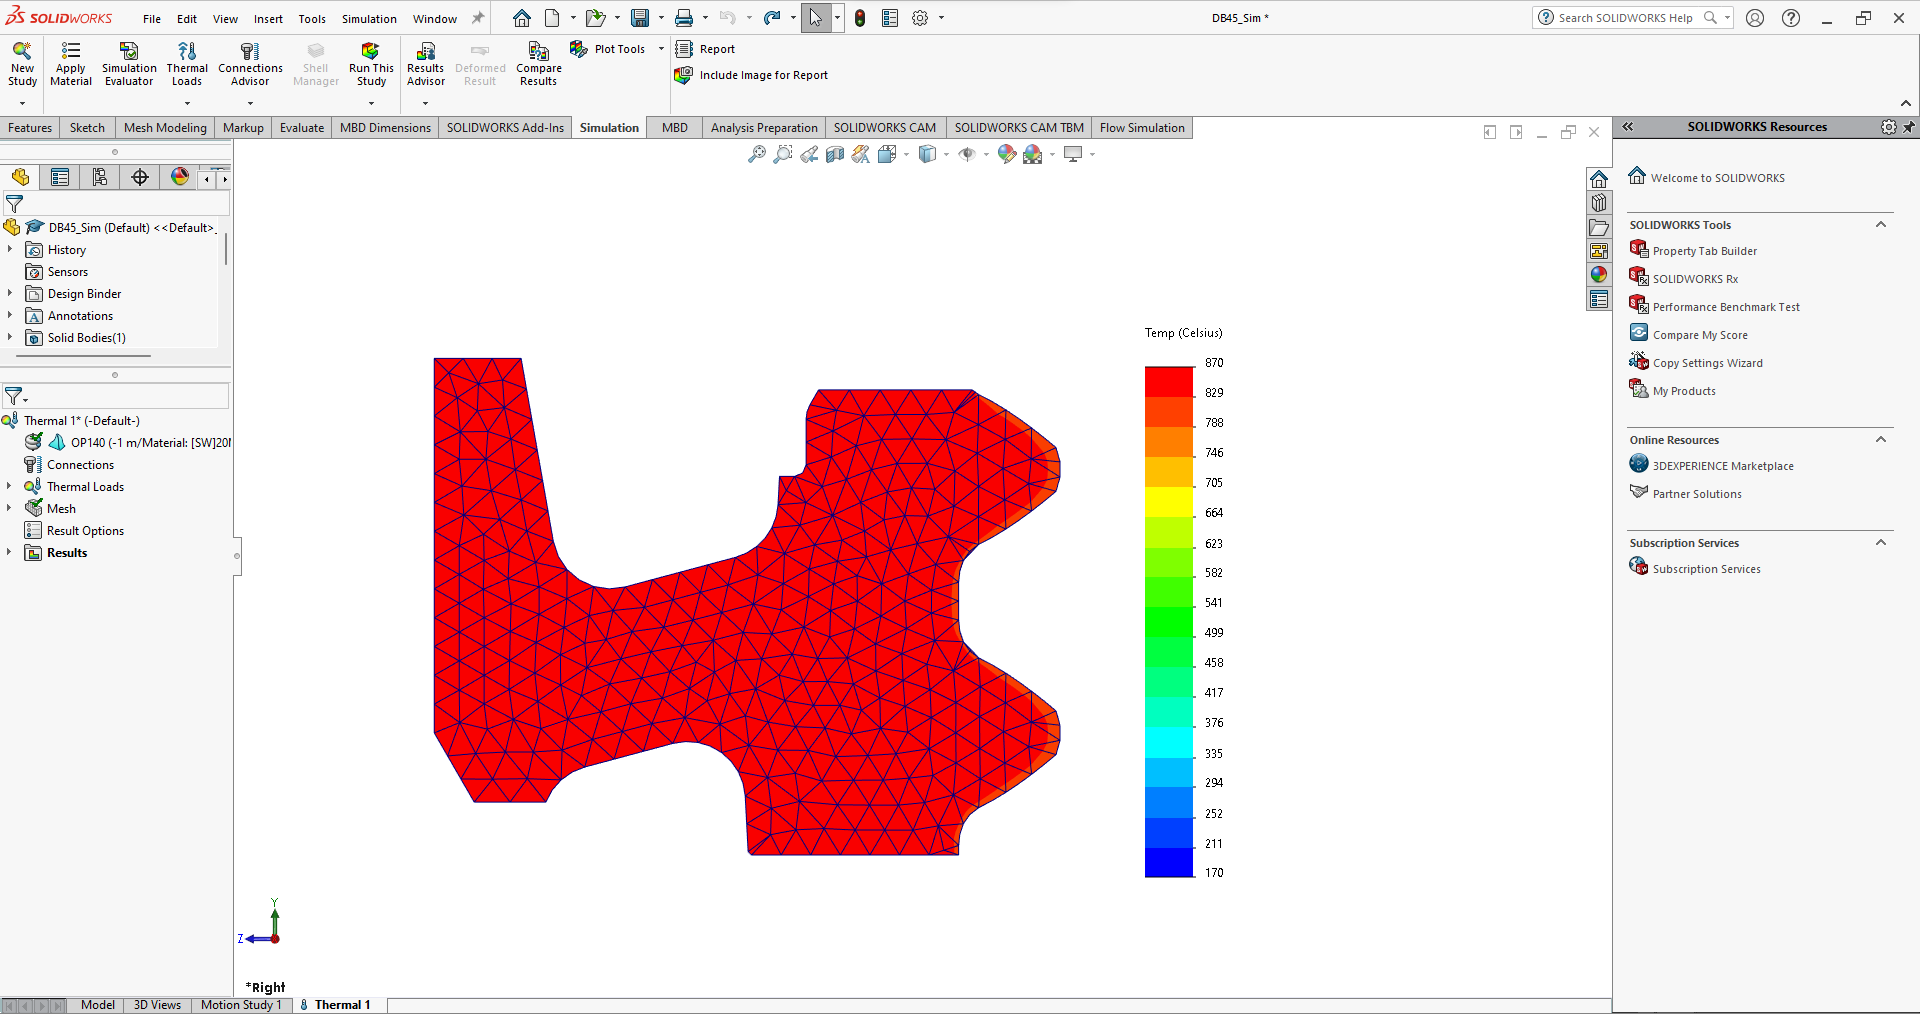
\includegraphics[width = 0.6\textwidth]{Figures/Cap4/Solidworks_thermal.png}
    \caption[Simulação puramente térmica Solidworks]%
    {Add-in do Solidworks simulation thermal para uma simulação puramente térmica.}
    \label{fig:simulacao_termica}
\end{figure}
%%%%%%%%%%%%%%%%%%%%%%%%%%%%%%%%%%%%%%%%%%%%%%%%%%%%%%%%%%%%%%%%%%%%%%%%%%%%%
\par
Concluída a simulação, foram obtidos os valores do tempo em seis pontos, três para o dentado e três para o diâmetro interno. O primeiro ponto, é obtido quando os elementos atingem o valor de temperatura de austenitização A3, o segundo ponto, quando os elementos atingem a temperatura de austenitização A1, por fim, o terceiro ponto, quando os elementos atingem a temperatura de 170 \textdegree C. As Figuras \ref{fig:Dentado} são referentes aos pontos de temperaturas do dentado, e as Figuras \ref{fig:Diametro}, referentes aos pontos de temperaturas do diâmetro interno das rodas de coroa.
De forma a facilitar a visualização, foi escolhida apenas a roda de coroa Nº 6, ou seja, a roda do meio da coluna, e as simulações foram feitas num modelo em corte por simetria, com elementos bidimensionais, com o objetivo de diminuir o número de elementos utilizados em cada simulação. A tabela \ref{tab:pontos_sim} indica os valores dos pontos e o tempo em cada um deles, que foram retirados das imagens. Com estes valores é então possível determinar a velocidade de arrefecimento nos pontos em questão e então estimar a microestrutura final no dentado e no diâmetro interno. Para além disso, é possível também prever a dureza final nos dois pontos, tendo em conta a microestrutura, a velocidade de arrefecimento e a composição química do material.
\newpage
%%%%%%%%%%%%%%%%%%%%%%%%%%%%%%%%%%%%%%%%%%%%%%%%%%%%%%%%%%%%%%%%%%%%%%%%%%%%%
\begin{figure}[htb]
    \centering
    \begin{subfigure}{.33\textwidth}\
        \centering
        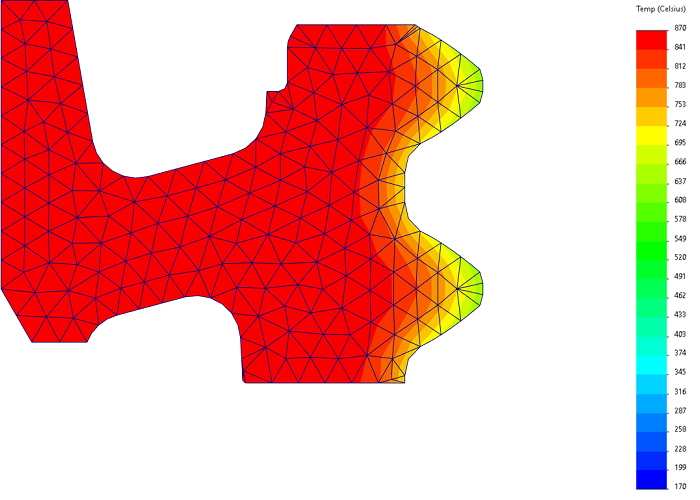
\includegraphics[width = 0.8\textwidth]{Figures/Cap4/AC3_Dentado.png}
        \caption[]%
        {}
        \label{fig:A3_Dent}
    \end{subfigure}%
    \begin{subfigure}{.33\textwidth}
        \centering
        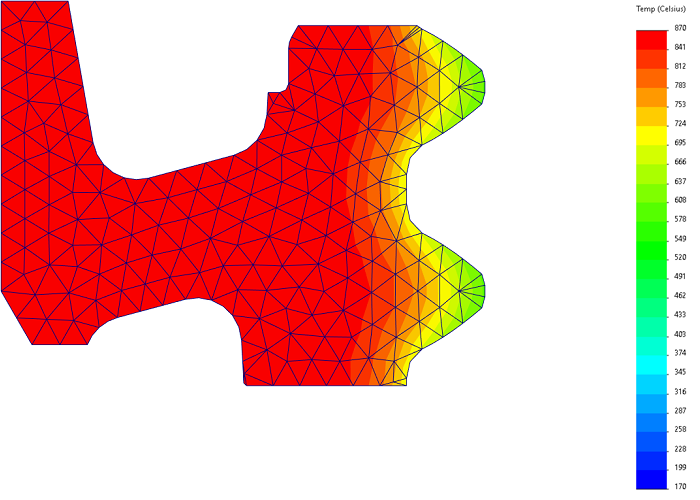
\includegraphics[width = 0.8\textwidth]{Figures/Cap4/AC1_Dentado.png}
        \caption{}
        \label{fig:A1_Dent}
    \end{subfigure}
    \begin{subfigure}{.33\textwidth}
        \centering
        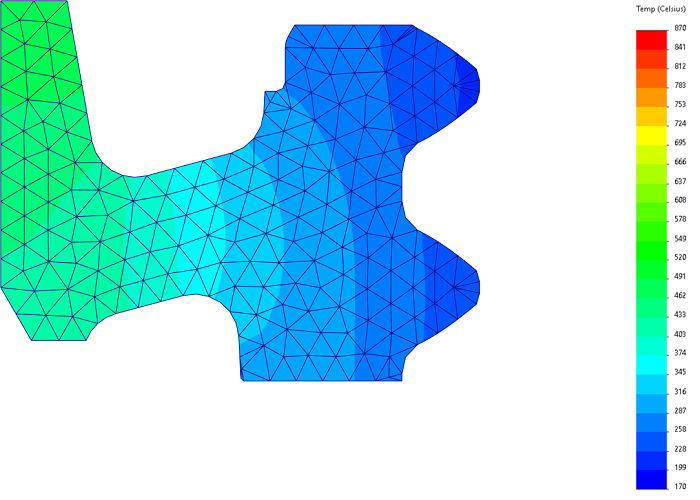
\includegraphics[width = 0.8\textwidth]{Figures/Cap4/TF_Dentado.png}
        \caption{}
        \label{fig:Tf_Dent}
    \end{subfigure}
    \caption[Pontos críticos dos elementos finitos do dentado]%
    {Pontos críticos dos elementos finitos do dentado, para obtenção dos valores de tempo. À esquerda, temperatura A\textsubscript{C1}, que ocorre aos 0,45s, no centro, temperatura A\textsubscript{C3}, que ocorre aos 3,05 s, e à direita, temperatura T\textsubscript{F}, aos 52,00s.}
    \label{fig:Dentado}
\end{figure}
%%%%%%%%%%%%%%%%%%%%%%%%%%%%%%%%%%%%%%%%%%%%%%%%%%%%%%%%%%%%%%%%%%%%%%%%%%%%%
%%%%%%%%%%%%%%%%%%%%%%%%%%%%%%%%%%%%%%%%%%%%%%%%%%%%%%%%%%%%%%%%%%%%%%%%%%%%%
\begin{figure}[htb]
    \centering
    \begin{subfigure}{.33\textwidth}\
        \centering
        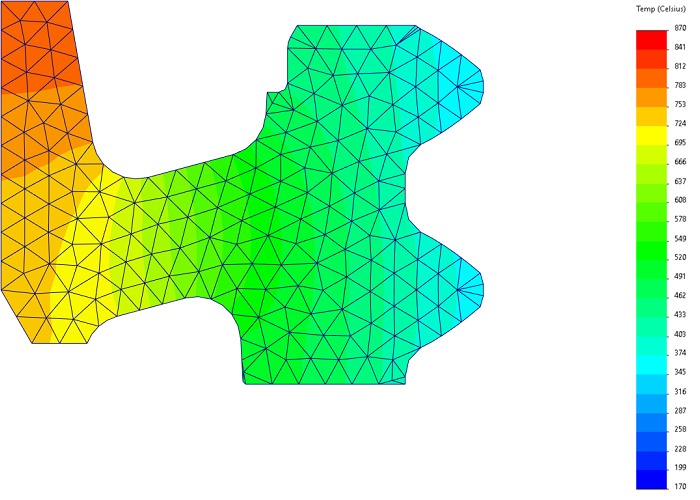
\includegraphics[width = 0.8\textwidth]{Figures/Cap4/AC3_Diametro.png}
        \caption[]%
        {}
        \label{fig:A3_Dint}
    \end{subfigure}%
    \begin{subfigure}{.33\textwidth}
        \centering
        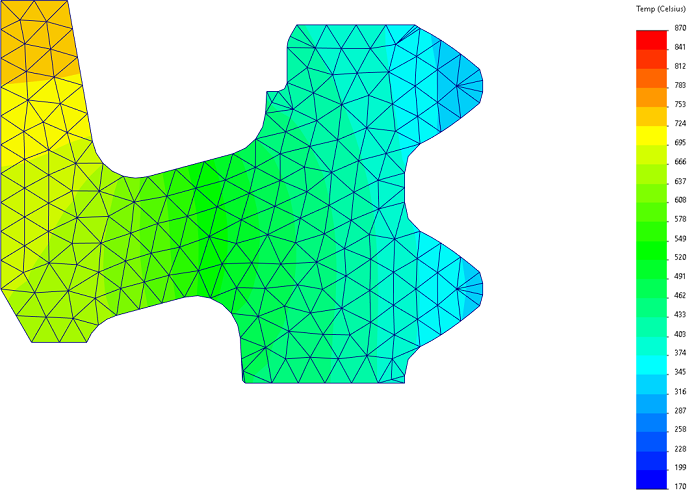
\includegraphics[width = 0.8\textwidth]{Figures/Cap4/AC1_Diametro.png}
        \caption{}
        \label{fig:A1_Dint}
    \end{subfigure}
    \begin{subfigure}{.33\textwidth}
        \centering
        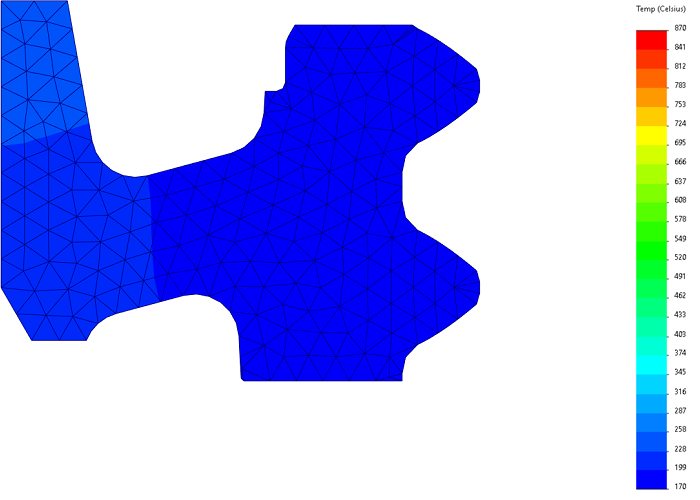
\includegraphics[width = 0.8\textwidth]{Figures/Cap4/TF_Diametro.png}
        \caption{}
        \label{fig:Tf_Dint}
    \end{subfigure}
    \caption[Pontos críticos dos elementos finitos do diâmetro interno]%
    {Pontos críticos dos elementos finitos do diâmetro interno, para obtenção dos valores de tempo. À esquerda, temperatura A\textsubscript{C1}, que ocorre aos 27,65s, no centro, temperatura A\textsubscript{C3}, que ocorre aos 47,15 s, e à direita, temperatura T\textsubscript{F}, aos 170,00s.}
    \label{fig:Diametro}
\end{figure}
%%%%%%%%%%%%%%%%%%%%%%%%%%%%%%%%%%%%%%%%%%%%%%%%%%%%%%%%%%%%%%%%%%%%%%%%%%%%%
\par
Observa-se que foi utilizada uma taxa de carbono de 0,7\% no dentado e 0,24\% no diâmetro interno, no entanto, é importante salientar que não se pode garantir a ausência de enriquecimento de carbono no diâmetro interno. Como não é possível prever o valor final da percentagem de carbono no diâmetro interno, optou-se por utilizar o valor do material base. Com base nos valores obtidos, é possível estimar uma velocidade média de arrefecimento de aproximadamente 35,0°C/s para o dentado e uma velocidade média de arrefecimento de 4,7°C/s para o diâmetro interno.
\par
Para o dentado, estima-se níveis de dureza em torno de 860HV para uma microestrutura predominantemente martensítica e 290HV para uma microestrutura predominantemente ferrítica e perlítica. Já para o diâmetro interno, considerando a ausência de enriquecimento, estima-se que uma estrutura predominantemente martensítica apresente níveis de dureza em torno de 500HV, enquanto uma estrutura predominantemente ferrítica e perlítica apresente aproximadamente 190HV de dureza.
%%%%%%%%%%%%%%%%%%%%%%%%%%%%%%%%%%%%%%%%%%%%%%%%%%%%%%%%%%%%%%%%%%%%%%%%%%%%%
\begin{table}[htb]
    \centering
    \refstepcounter{table}
    \caption[Valores temporais para cada temperatura crítica]{Valores temporais para cada temperatura crítica no dentado e no diâmetro interno.}
    \label{tab:pontos_sim}
    \begin{tabular}{lr} 
    \toprule
    \multicolumn{1}{c}{\textbf{Ponto Crítico}}            & \multicolumn{1}{c}{\textbf{Tempo (s)}}                         \\ 
    \hline\hline
    Início de Têmpera (T\textsubscript{0})                                & 0,00 s                                         \\ 
    \hline
    Final de Austenitização no dentado (A\textsubscript{C3\_t})           & 0,45 s                                         \\
    Início de Austenitização no dentado (A\textsubscript{C1\_t})          & 3,05 s                                         \\
    Final de Têmpera no dentado (T\textsubscript{F\_t})                   & 52,00 s                                        \\ 
    \hline\hline
    Final de Austenitização no dentado (A\textsubscript{C3\_t})           & 27,65 s                                        \\
    Início de Austenitização no diâmetro interno (A\textsubscript{C1\_d}) & 47,15 s                                        \\ 
    Final de Têmpera (T\textsubscript{F\_d})                              & 170,00 s                                       \\
    \bottomrule
    \end{tabular}
\end{table}
%%%%%%%%%%%%%%%%%%%%%%%%%%%%%%%%%%%%%%%%%%%%%%%%%%%%%%%%%%%%%%%%%%%%%%%%%%%%%
\par
Uma vez que, para as velocidades de arrefecimento em questão, espera-se que o dentado apresente principalmente martensite, enquanto o diâmetro interno apresenta ferrite e perlite, é esperado que as durezas estejam em torno de 860HV para o dentado e 190HV para o diâmetro interno. No entanto, é importante ressaltar que essas estimativas são para o material que não passou pelo processo de revenido, no caso do dentado, e não sofreu enriquecimento de carbono, no caso do diâmetro interno. Caso o material seja submetido ao processo de revenido, espera-se uma redução nos níveis de dureza. De maneira análoga, caso ocorra enriquecimento de carbono no diâmetro interno, espera-se um aumento nos níveis de dureza.

%%%%%%%%%%%%%%%%%%%%%%%%%%%%%%%%%%%%%%%%%%%%%%%%%%%%%%%%%%%%%%%%%%%%%%%%%%%%%
\section{Resultados do ensaio inicial} \label{sec:resultados_ensaio_inicial}

Conforme mencionado no Capítulo \ref{ch:materiais}, os resultados do protótipo inicial, mais especificamente da coluna protegida pela tampa P, ficaram aquém do esperado. A hipótese levantada para explicar esses resultados é que os três pontos de soldadura utilizados para unir a falsa coroa à torre, e isolar o diâmetro interno das coroas nessa coluna, sofreram rotura provavelmente devido à expansão térmica. De qualquer forma, as Figuras \ref{fig:resultados_Tampa_P_inicial} e \ref{fig:resultados_Serie_inicial} ilustram a diferença entre ter o diâmetro interno tamponado, e livre para a passagem do fluido de têmpera. Além disso, conforme observado nas Figuras \ref{fig:resultados_Tampa_P_inicial_dent} e \ref{fig:resultados_Serie_inicial_dent}, também é possível notar que o tamponamento do diâmetro interno não causa alterações significativas na dureza do dentado, o que confirma as vantagens da existência de uma ferramenta que protege o diâmetro interno das rodas de coroa.
%%%%%%%%%%%%%%%%%%%%%%%%%%%%%%%%%%%%%%%%%%%%%%%%%%%%%%%%%%%%%%%%%%%%%%%%%%%%%
\begin{figure}[htb]
    \centering
    \begin{subfigure}{.4\textwidth}
        \centering
        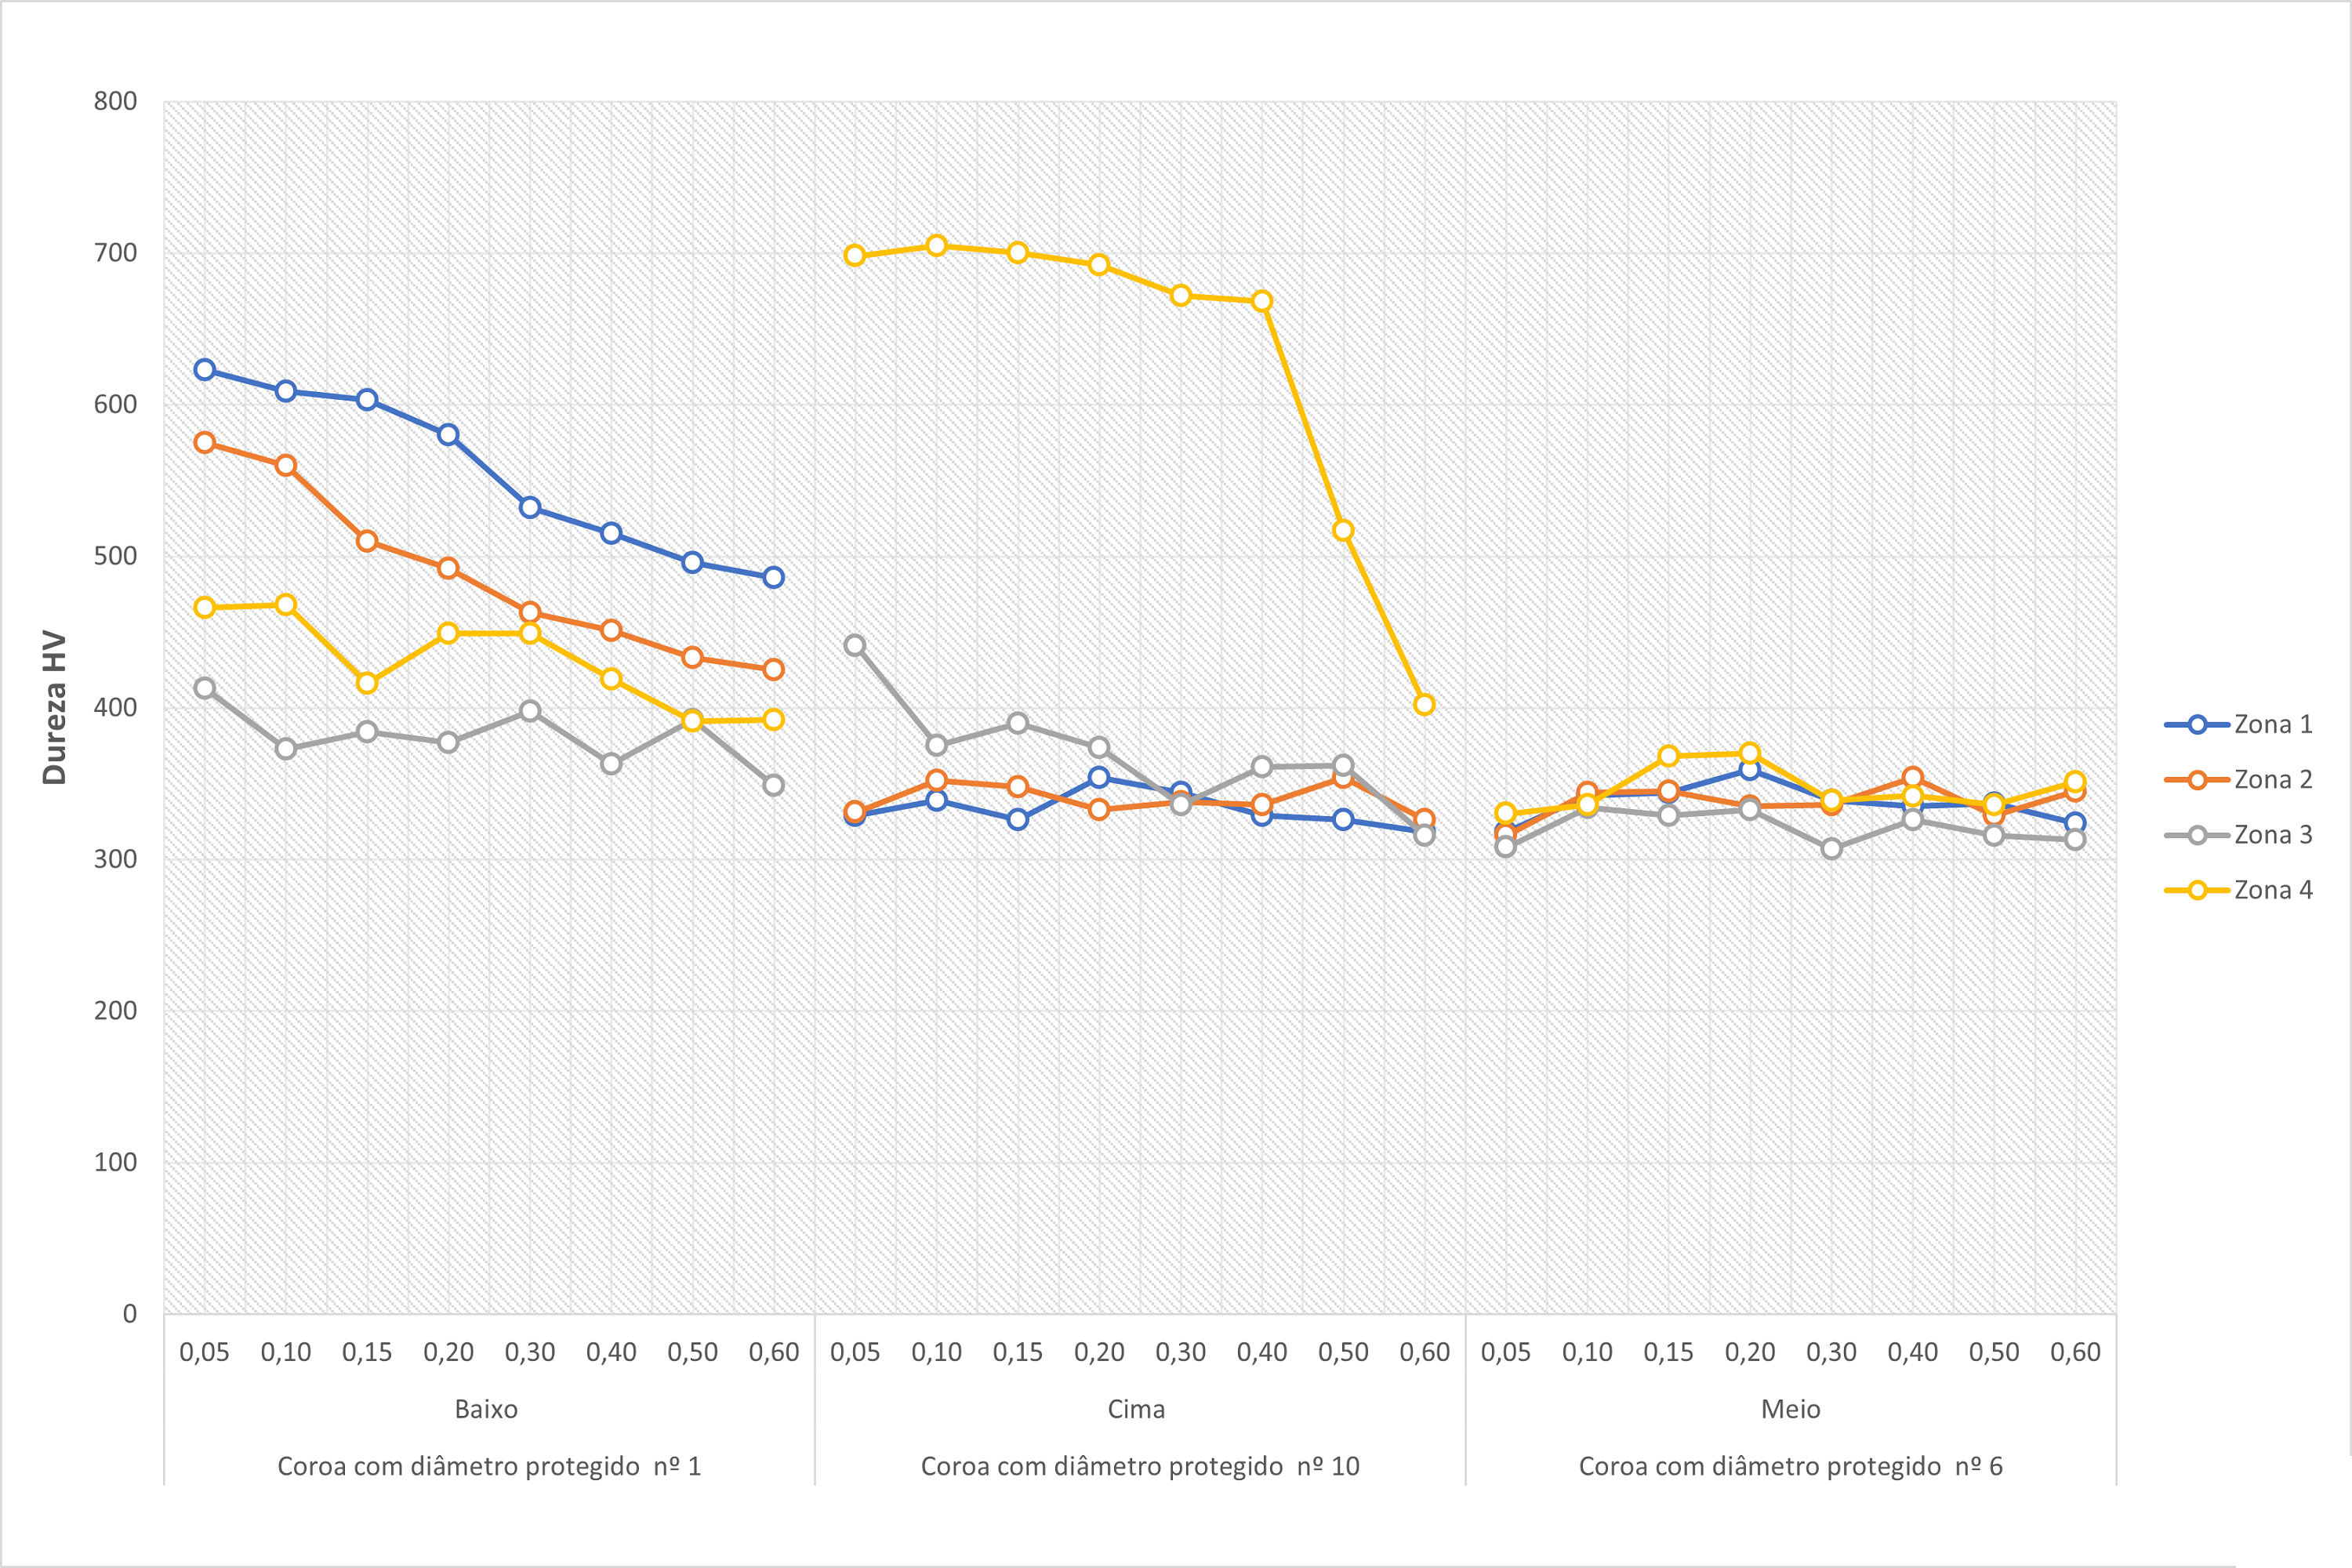
\includegraphics[width = 0.9\textwidth]{Figures/Cap4/Grafico_4_Zonas_P_inicial.png}
        \caption[]%
        {}
        \label{fig:resultados_Tampa_P_inicial}
    \end{subfigure}%
    \begin{subfigure}{.4\textwidth}
        \centering
        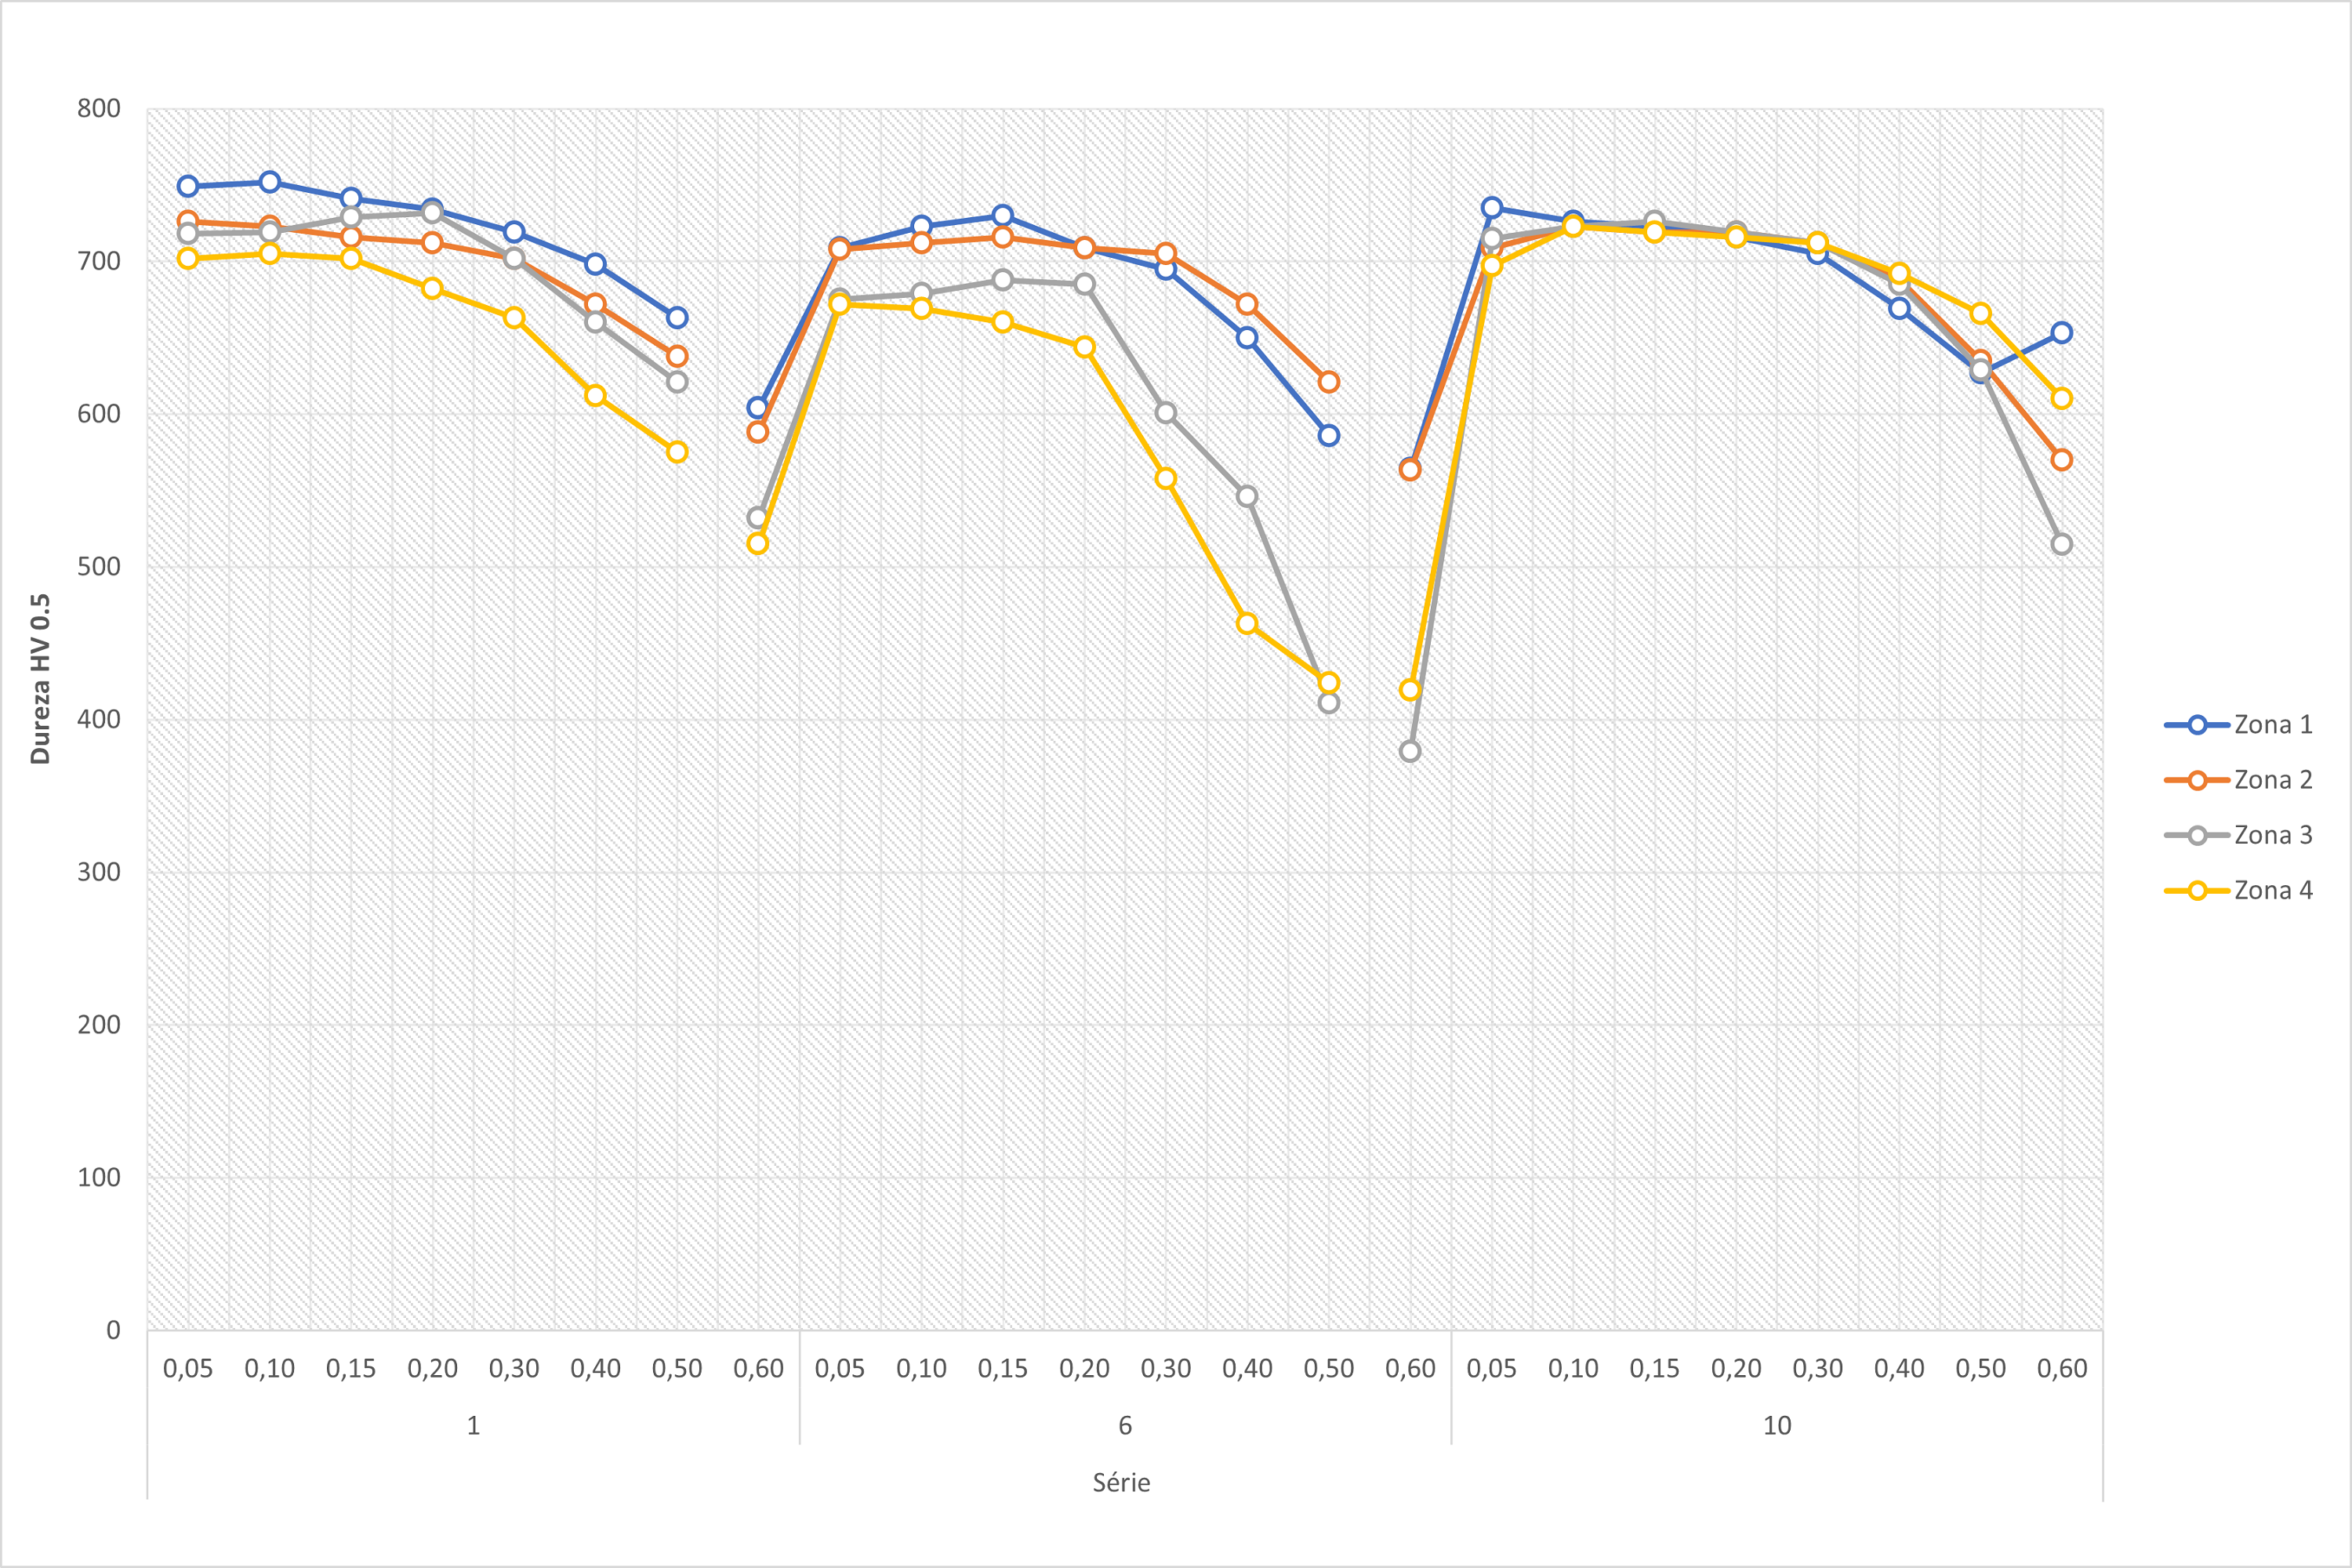
\includegraphics[width = 0.9\textwidth]{Figures/Cap4/Grafico_4_Zonas_S_inicial.png}
        \caption{}
        \label{fig:resultados_Serie_inicial}
    \end{subfigure}
    \begin{subfigure}{.4\textwidth}
        \centering
        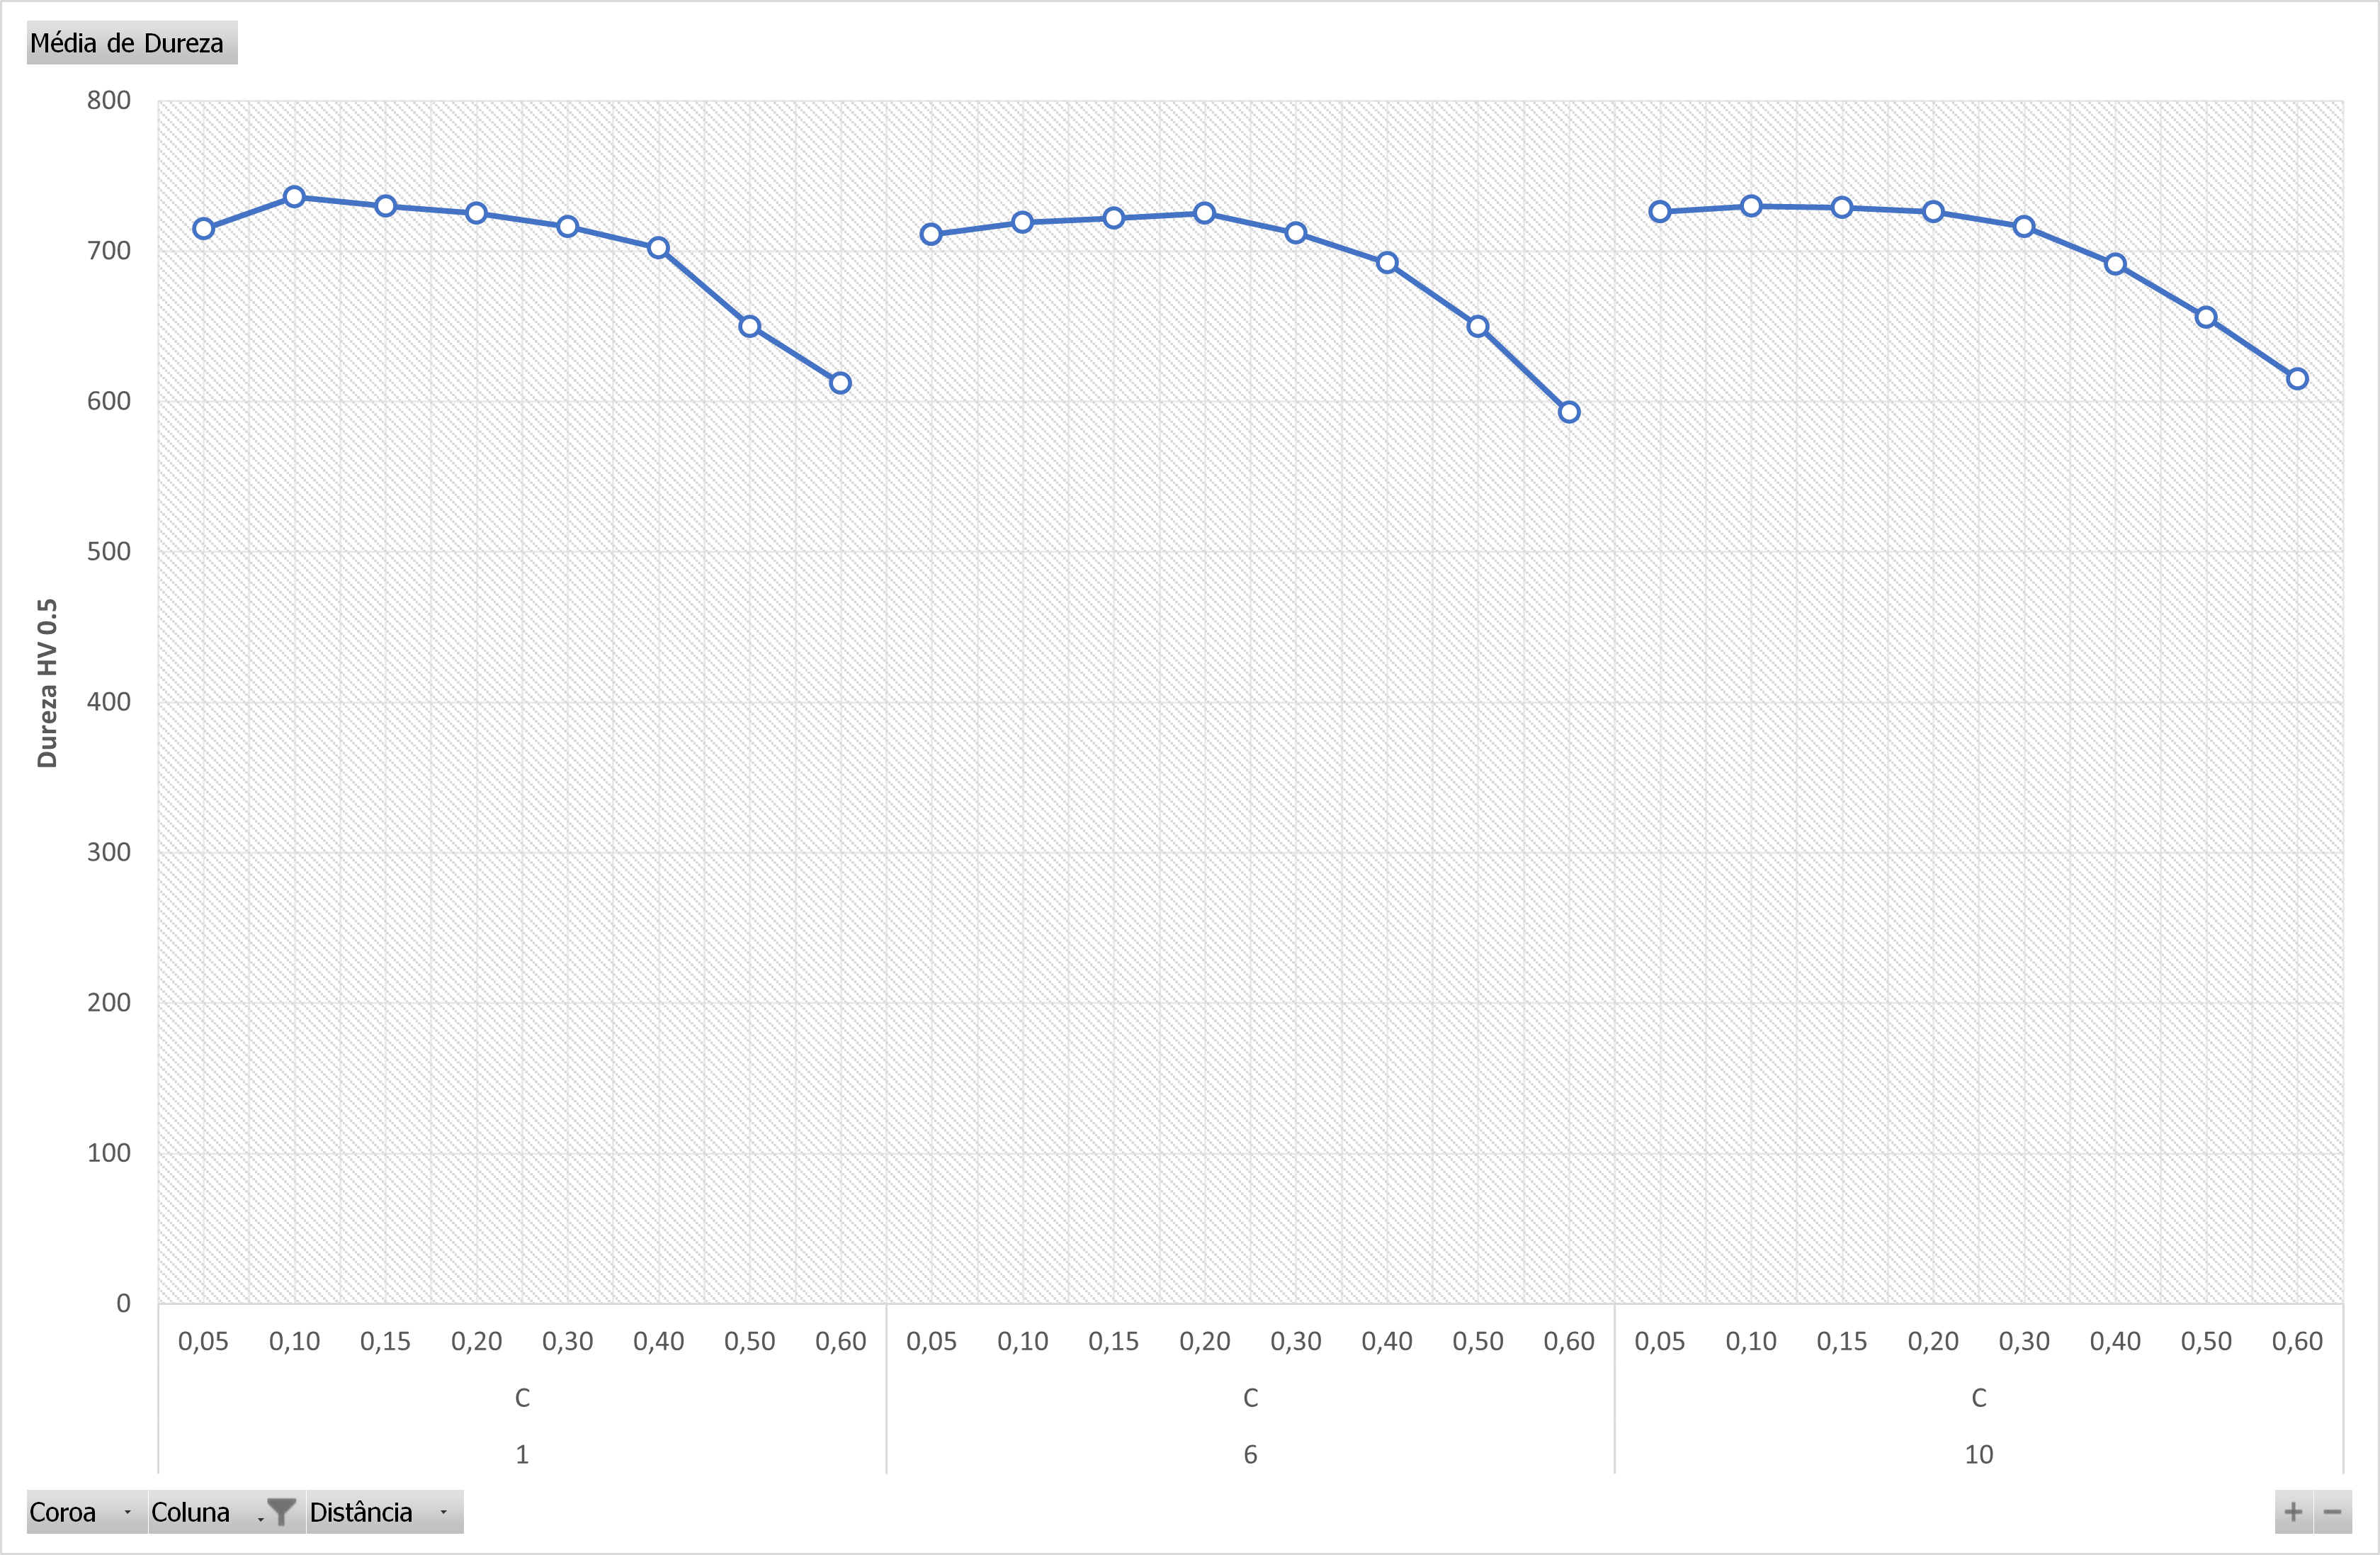
\includegraphics[width = 0.9\textwidth]{Figures/Cap4/Grafico_4_Zonas_P_inicial_dentado.png}
        \caption[]%
        {}
        \label{fig:resultados_Tampa_P_inicial_dent}
    \end{subfigure}%
    \begin{subfigure}{.4\textwidth}
        \centering
        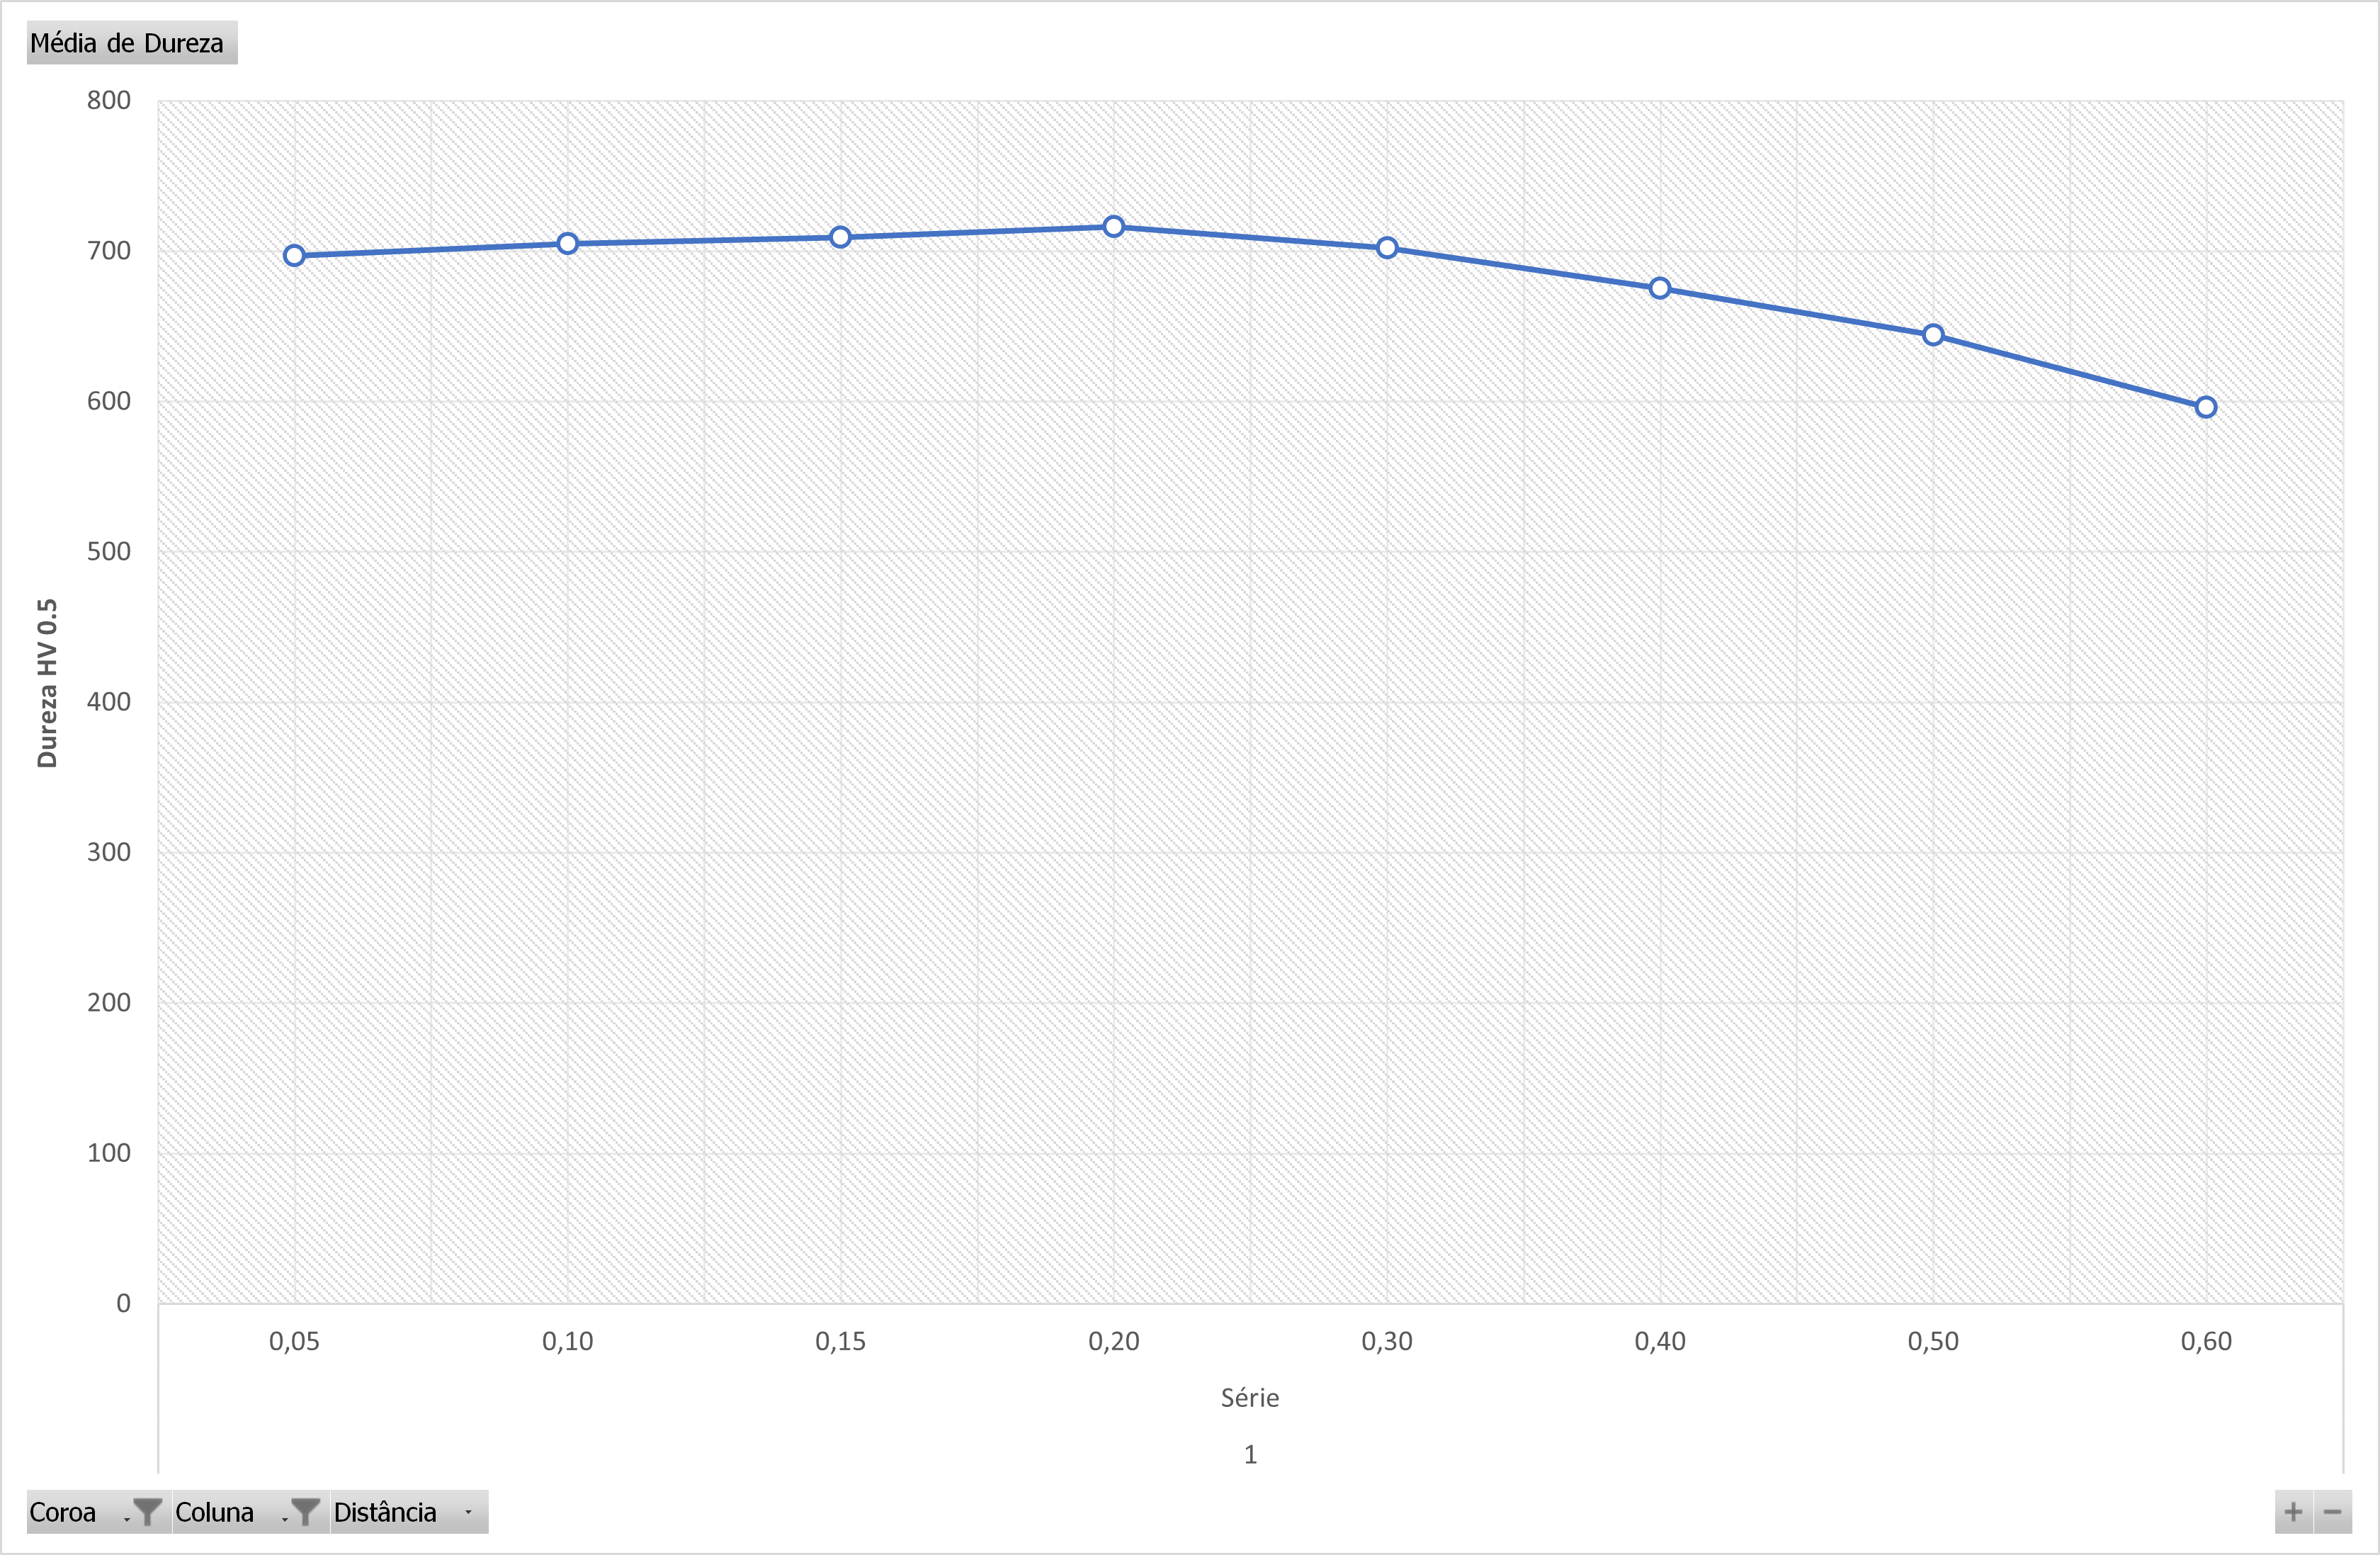
\includegraphics[width = 0.9\textwidth]{Figures/Cap4/Grafico_4_Zonas_S_inicial_dentado.png}
        \caption{}
        \label{fig:resultados_Serie_inicial_dent}
    \end{subfigure}
    \caption[Resultados do ensaio inicial e comparação com peças de série]%
    {Resultados das filiações de dureza obtidas no ensaio inicial, no diâmetro interno e no dentado, e comparação dos valores obtidos nos mesmos pontos nas peças de série.}
\end{figure}
%%%%%%%%%%%%%%%%%%%%%%%%%%%%%%%%%%%%%%%%%%%%%%%%%%%%%%%%%%%%%%%%%%%%%%%%%%%%%
\newpage
\par
É importante destacar que os valores de dureza encontrados no diâmetro interno estão consideravelmente acima dos valores teoricamente estimados, o que reforça a teoria de que há um enriquecimento de carbono nessa região das rodas de coroa protegidas. Outro fator relevante a ser mencionado é o ganho significativo de dureza na zona 4 da roda de coroa superior (número 1). Isso pode ser explicado pela geometria da tampa P, que faz contacto apenas nessa região, resultando em proteção parcial. Essa situação também explica a queda drástica na dureza a partir de 0,40 mm de profundidade. Por fim, observa-se o impacto da rotura da soldadura da falsa coroa na torre da ferramenta porta-peças. Isso permite uma passagem significativa de fluido de têmpera, causando um aumento expressivo nos níveis de dureza da roda de coroa inferior.
%%%%%%%%%%%%%%%%%%%%%%%%%%%%%%%%%%%%%%%%%%%%%%%%%%%%%%%%%%%%%%%%%%%%%%%%%%%%%
\section{Resultados dos ensaios nos protótipos aprimorados} \label{sec:resultados_ensaios}

Considerando que os resultados da tampa P foram influenciados pelos "defeitos" mencionados na secção anterior, apresentam-se os resultados das ferramentas aprimoradas, incluindo os resultados da tampa P após a soldadura completa da falsa coroa na torre. Novamente, para fins de comparação com os dados das peças de série, os dados das Figuras \ref{fig:resultados_Serie_inicial} e \ref{fig:resultados_Serie_inicial_dent} devem ser visualizados.
%%%%%%%%%%%%%%%%%%%%%%%%%%%%%%%%%%%%%%%%%%%%%%%%%%%%%%%%%%%%%%%%%%%%%%%%%%%%%
\begin{figure}[htb]
    \centering
    \begin{subfigure}{.4\textwidth}\
        \centering
        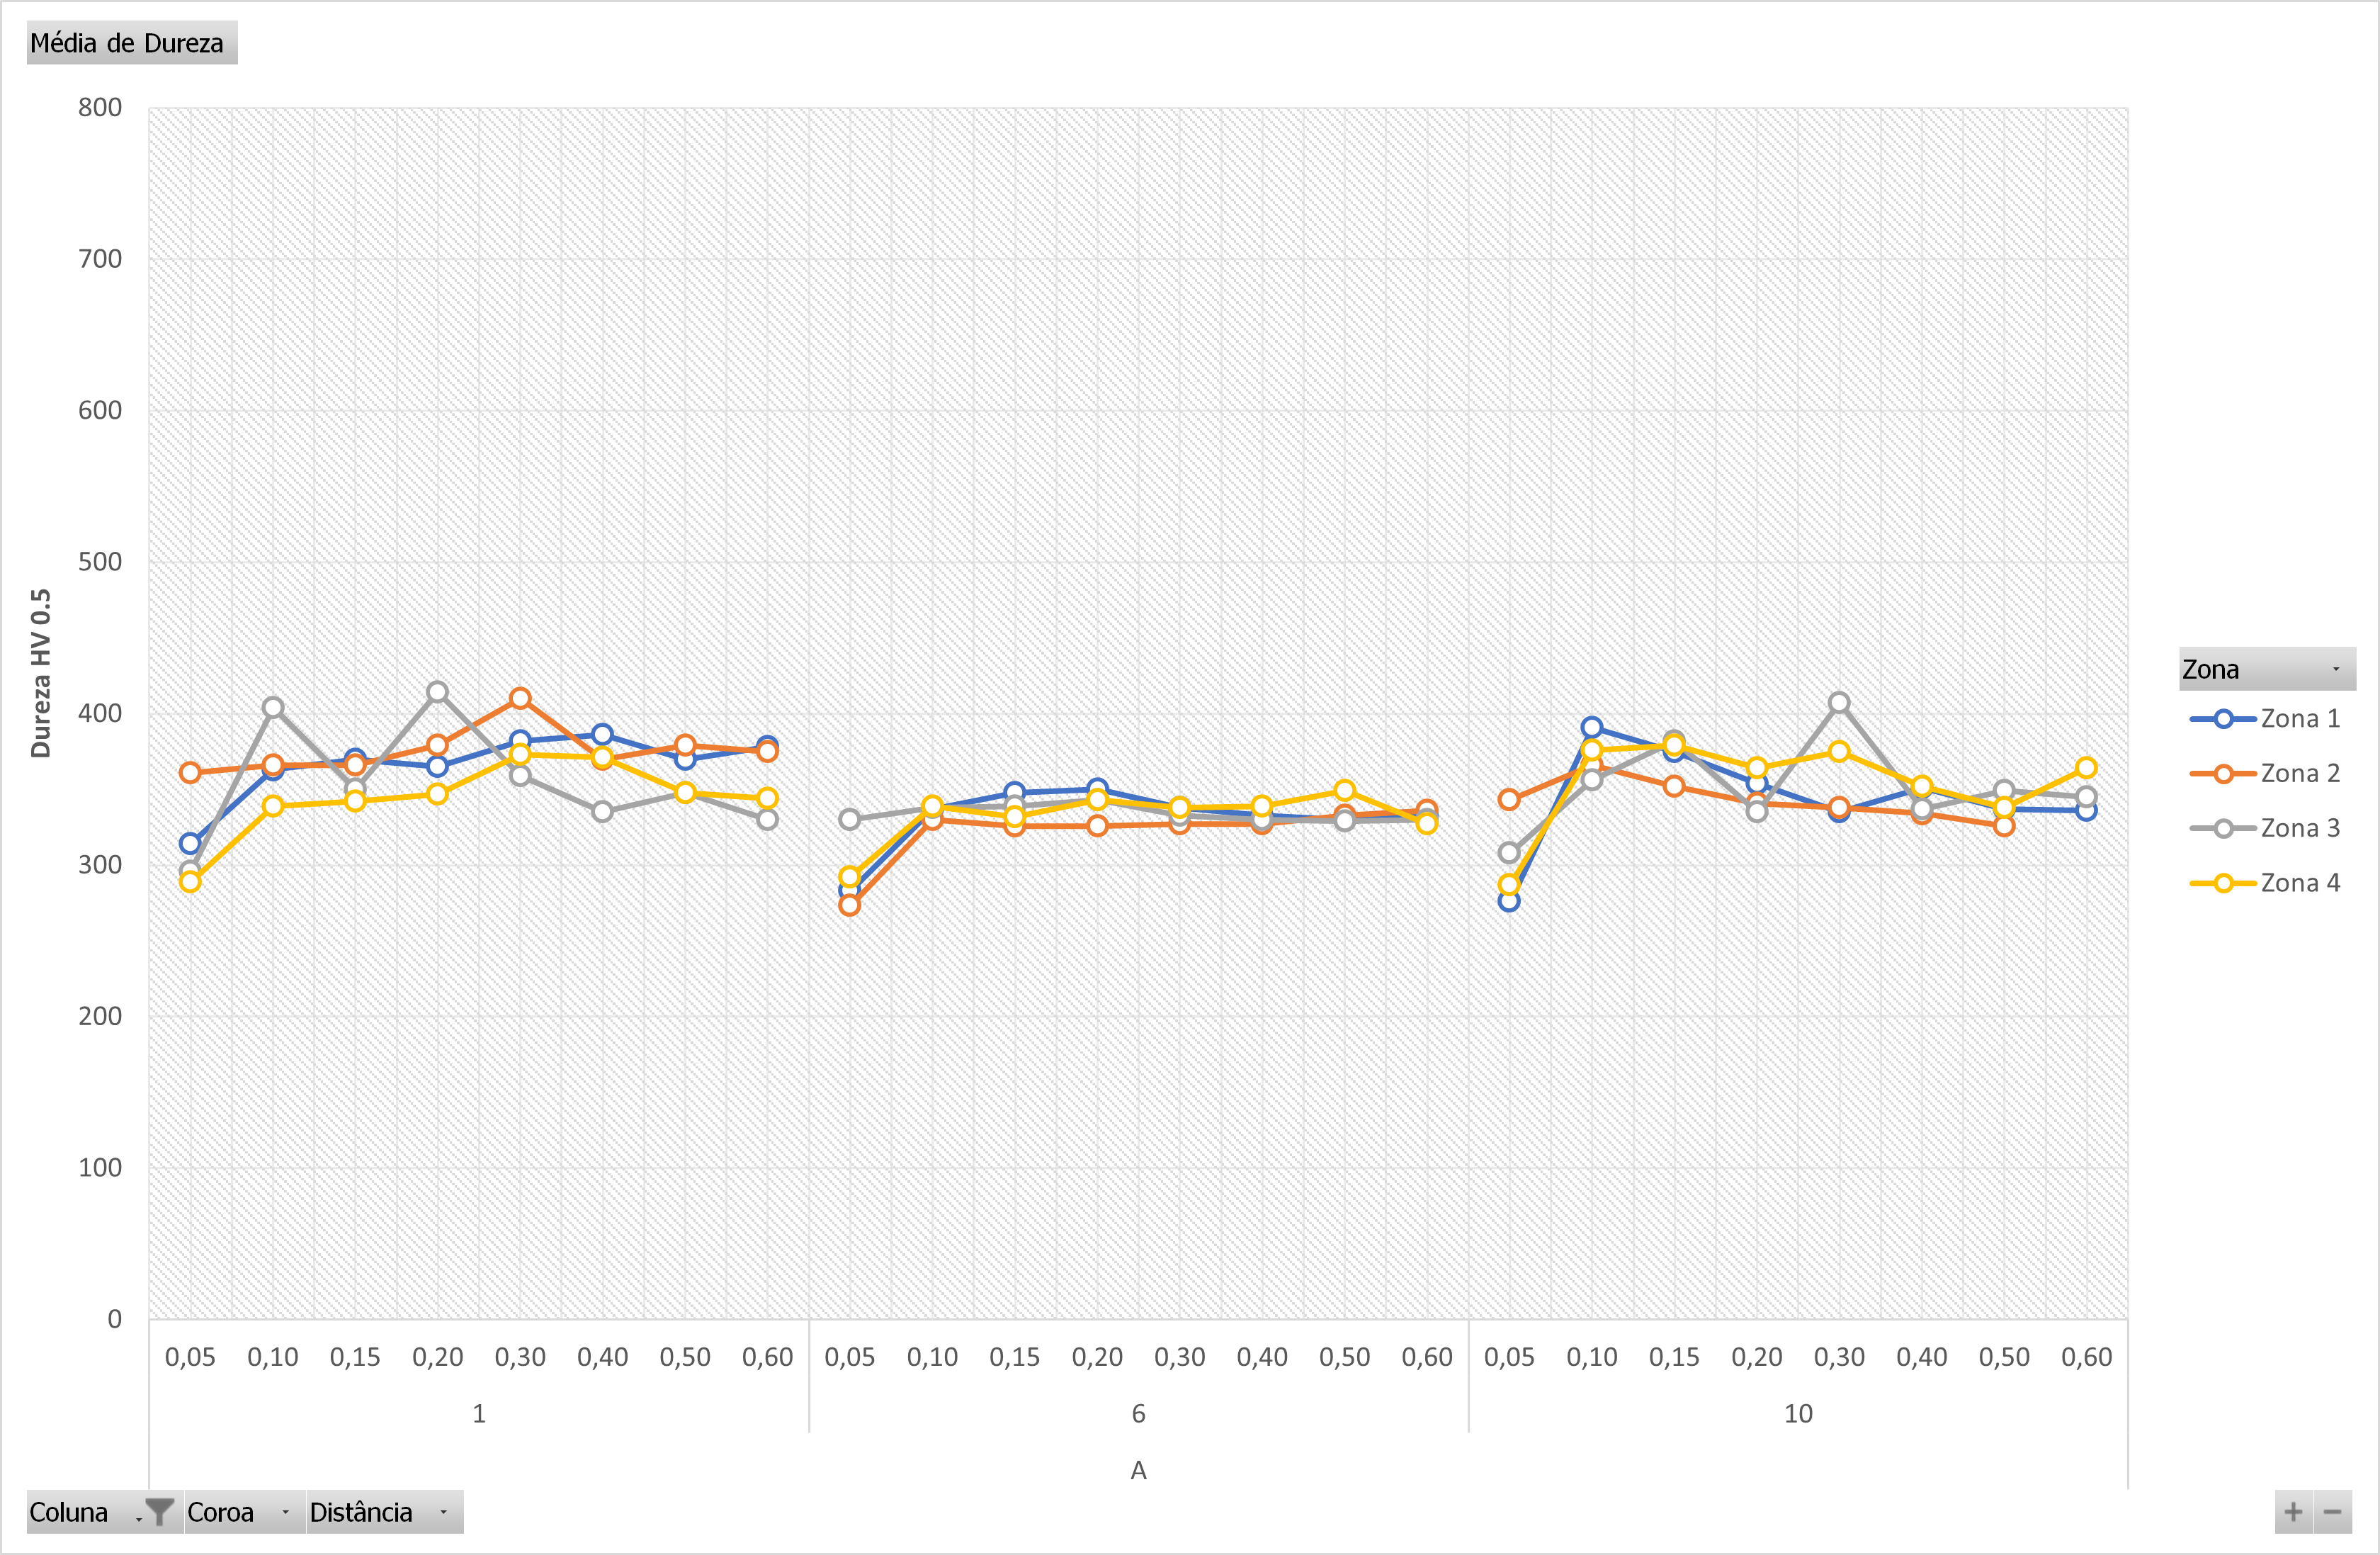
\includegraphics[width = 0.9\textwidth]{Figures/Cap4/Grafico_4_Zonas_Y.png}
        \caption{}
        \label{fig:resultados_Tampa_Y}
    \end{subfigure}%
    \begin{subfigure}{.4\textwidth}
        \centering
        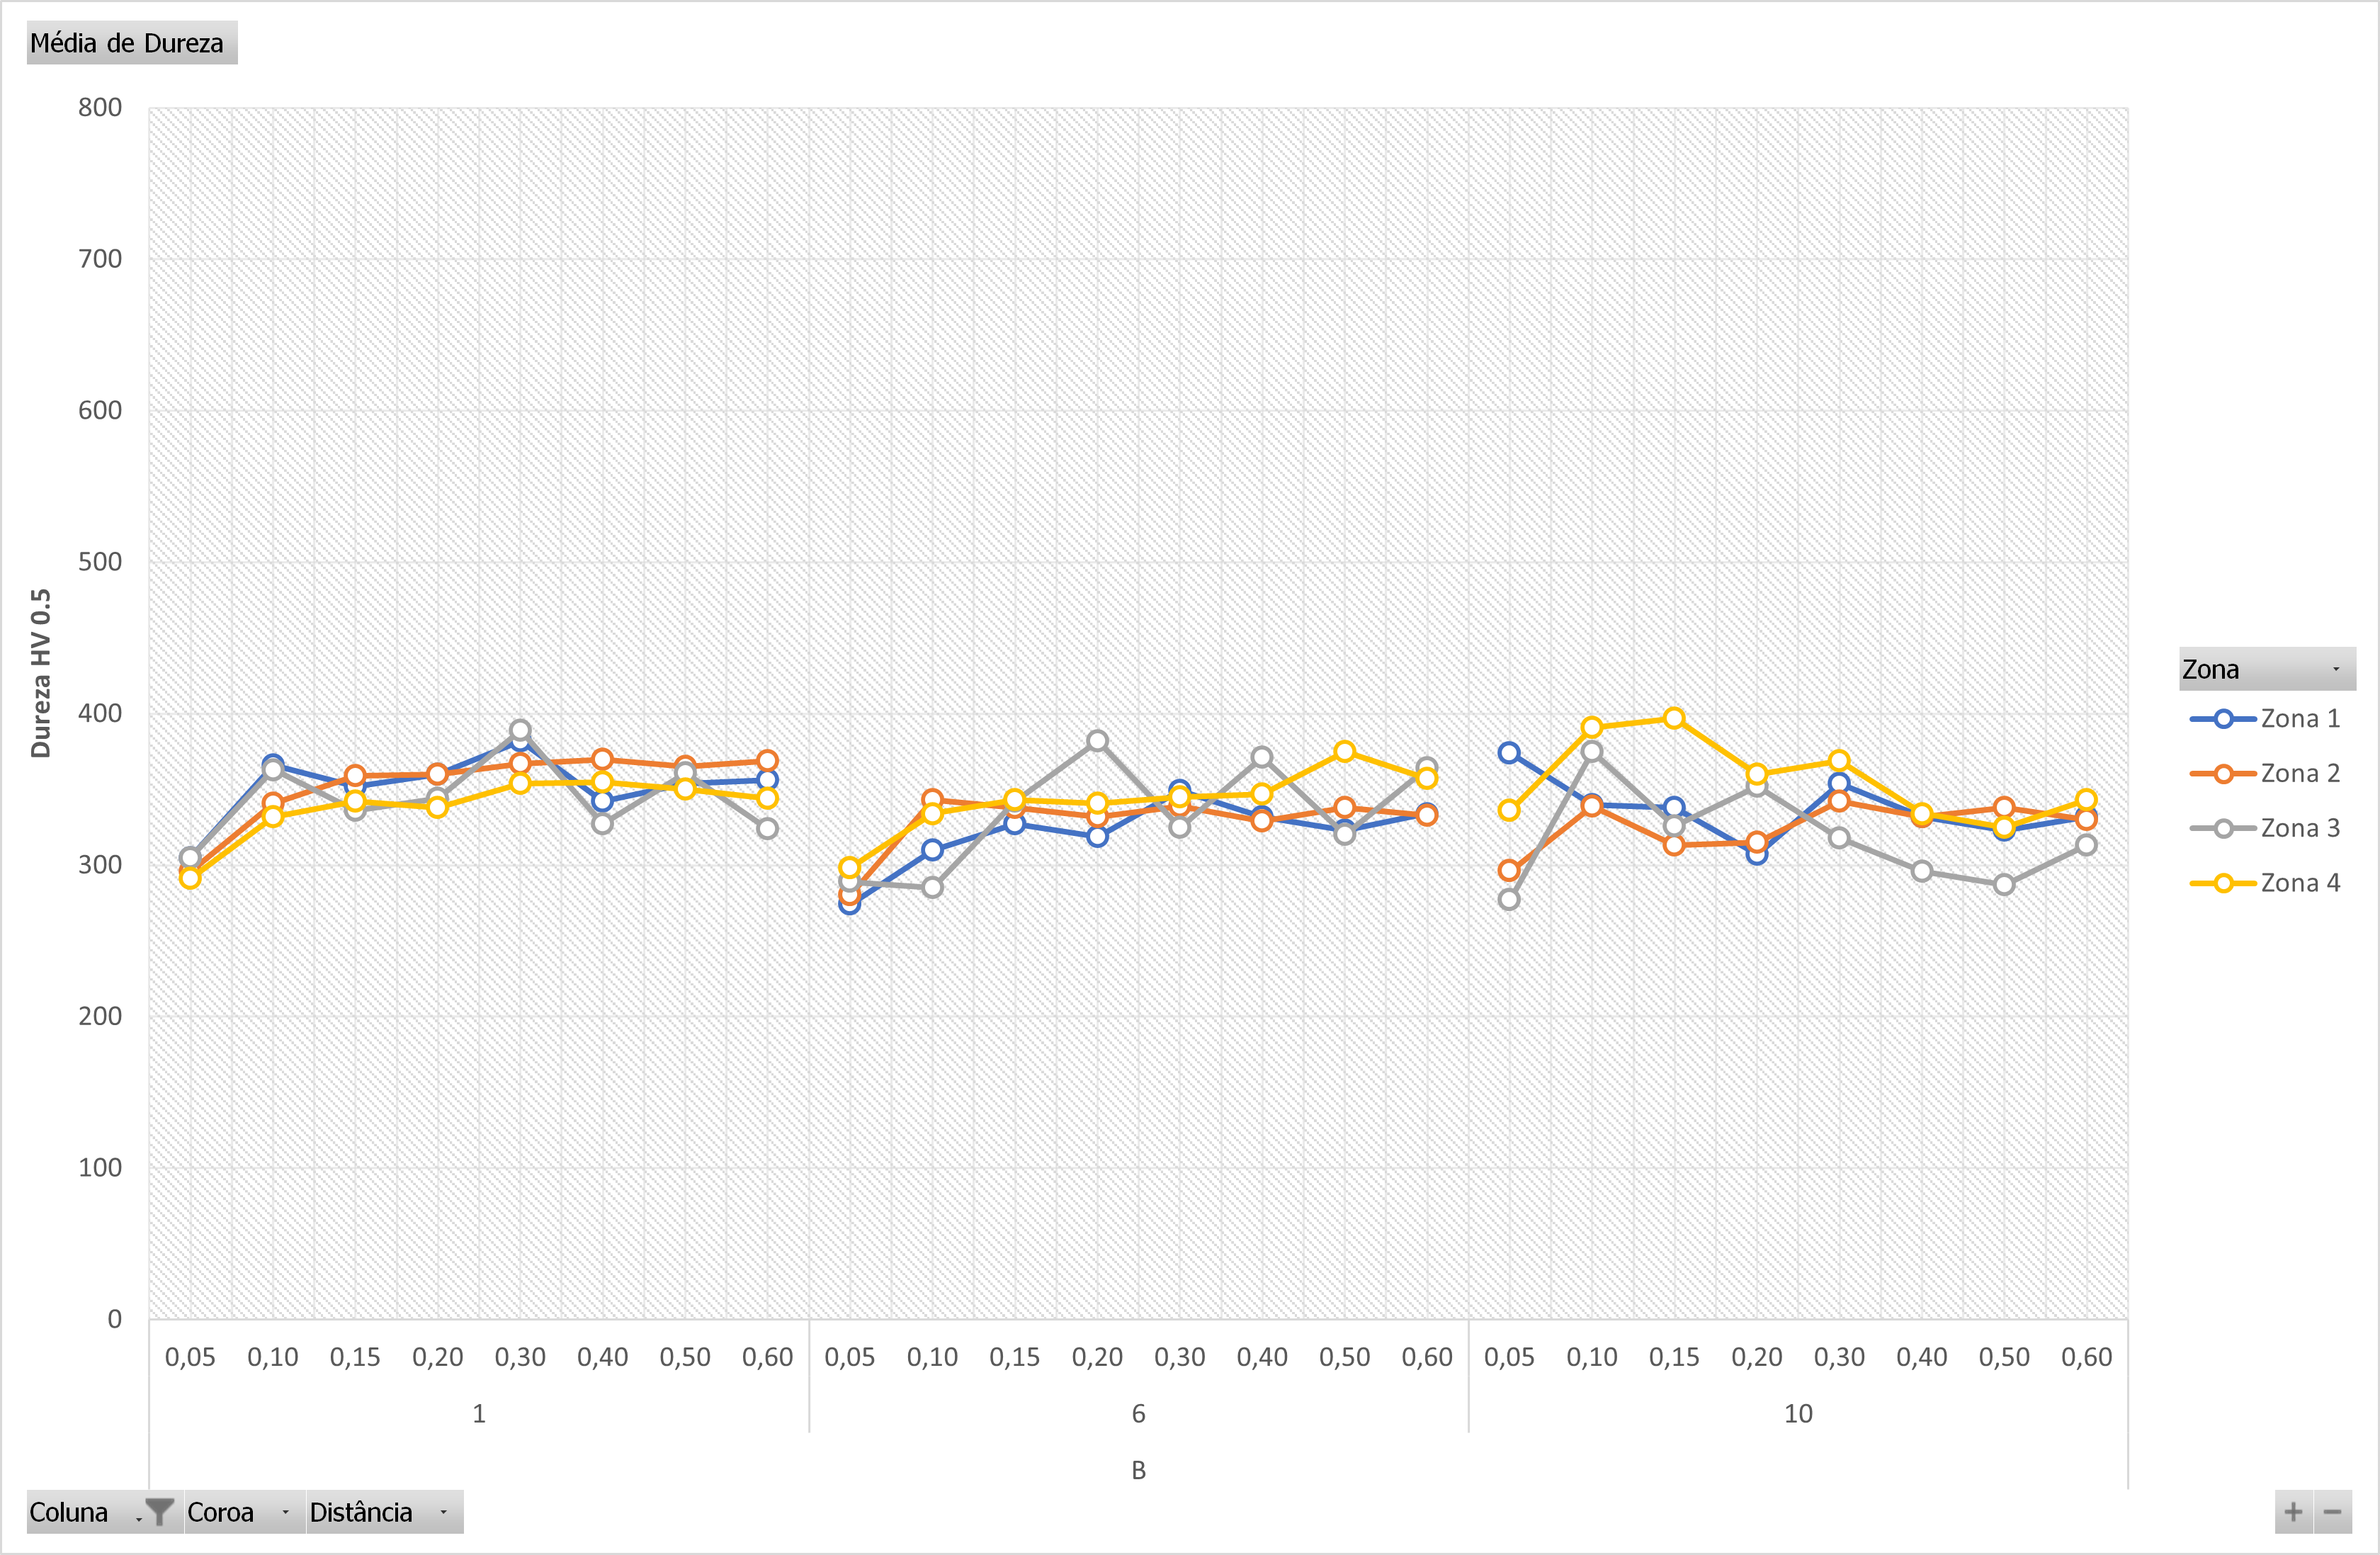
\includegraphics[width = 0.9\textwidth]{Figures/Cap4/Grafico_4_Zonas_O.png}
        \caption{}
        \label{fig:resultados_Tampa_O}
    \end{subfigure}
    \begin{subfigure}{.4\textwidth}\
        \centering
        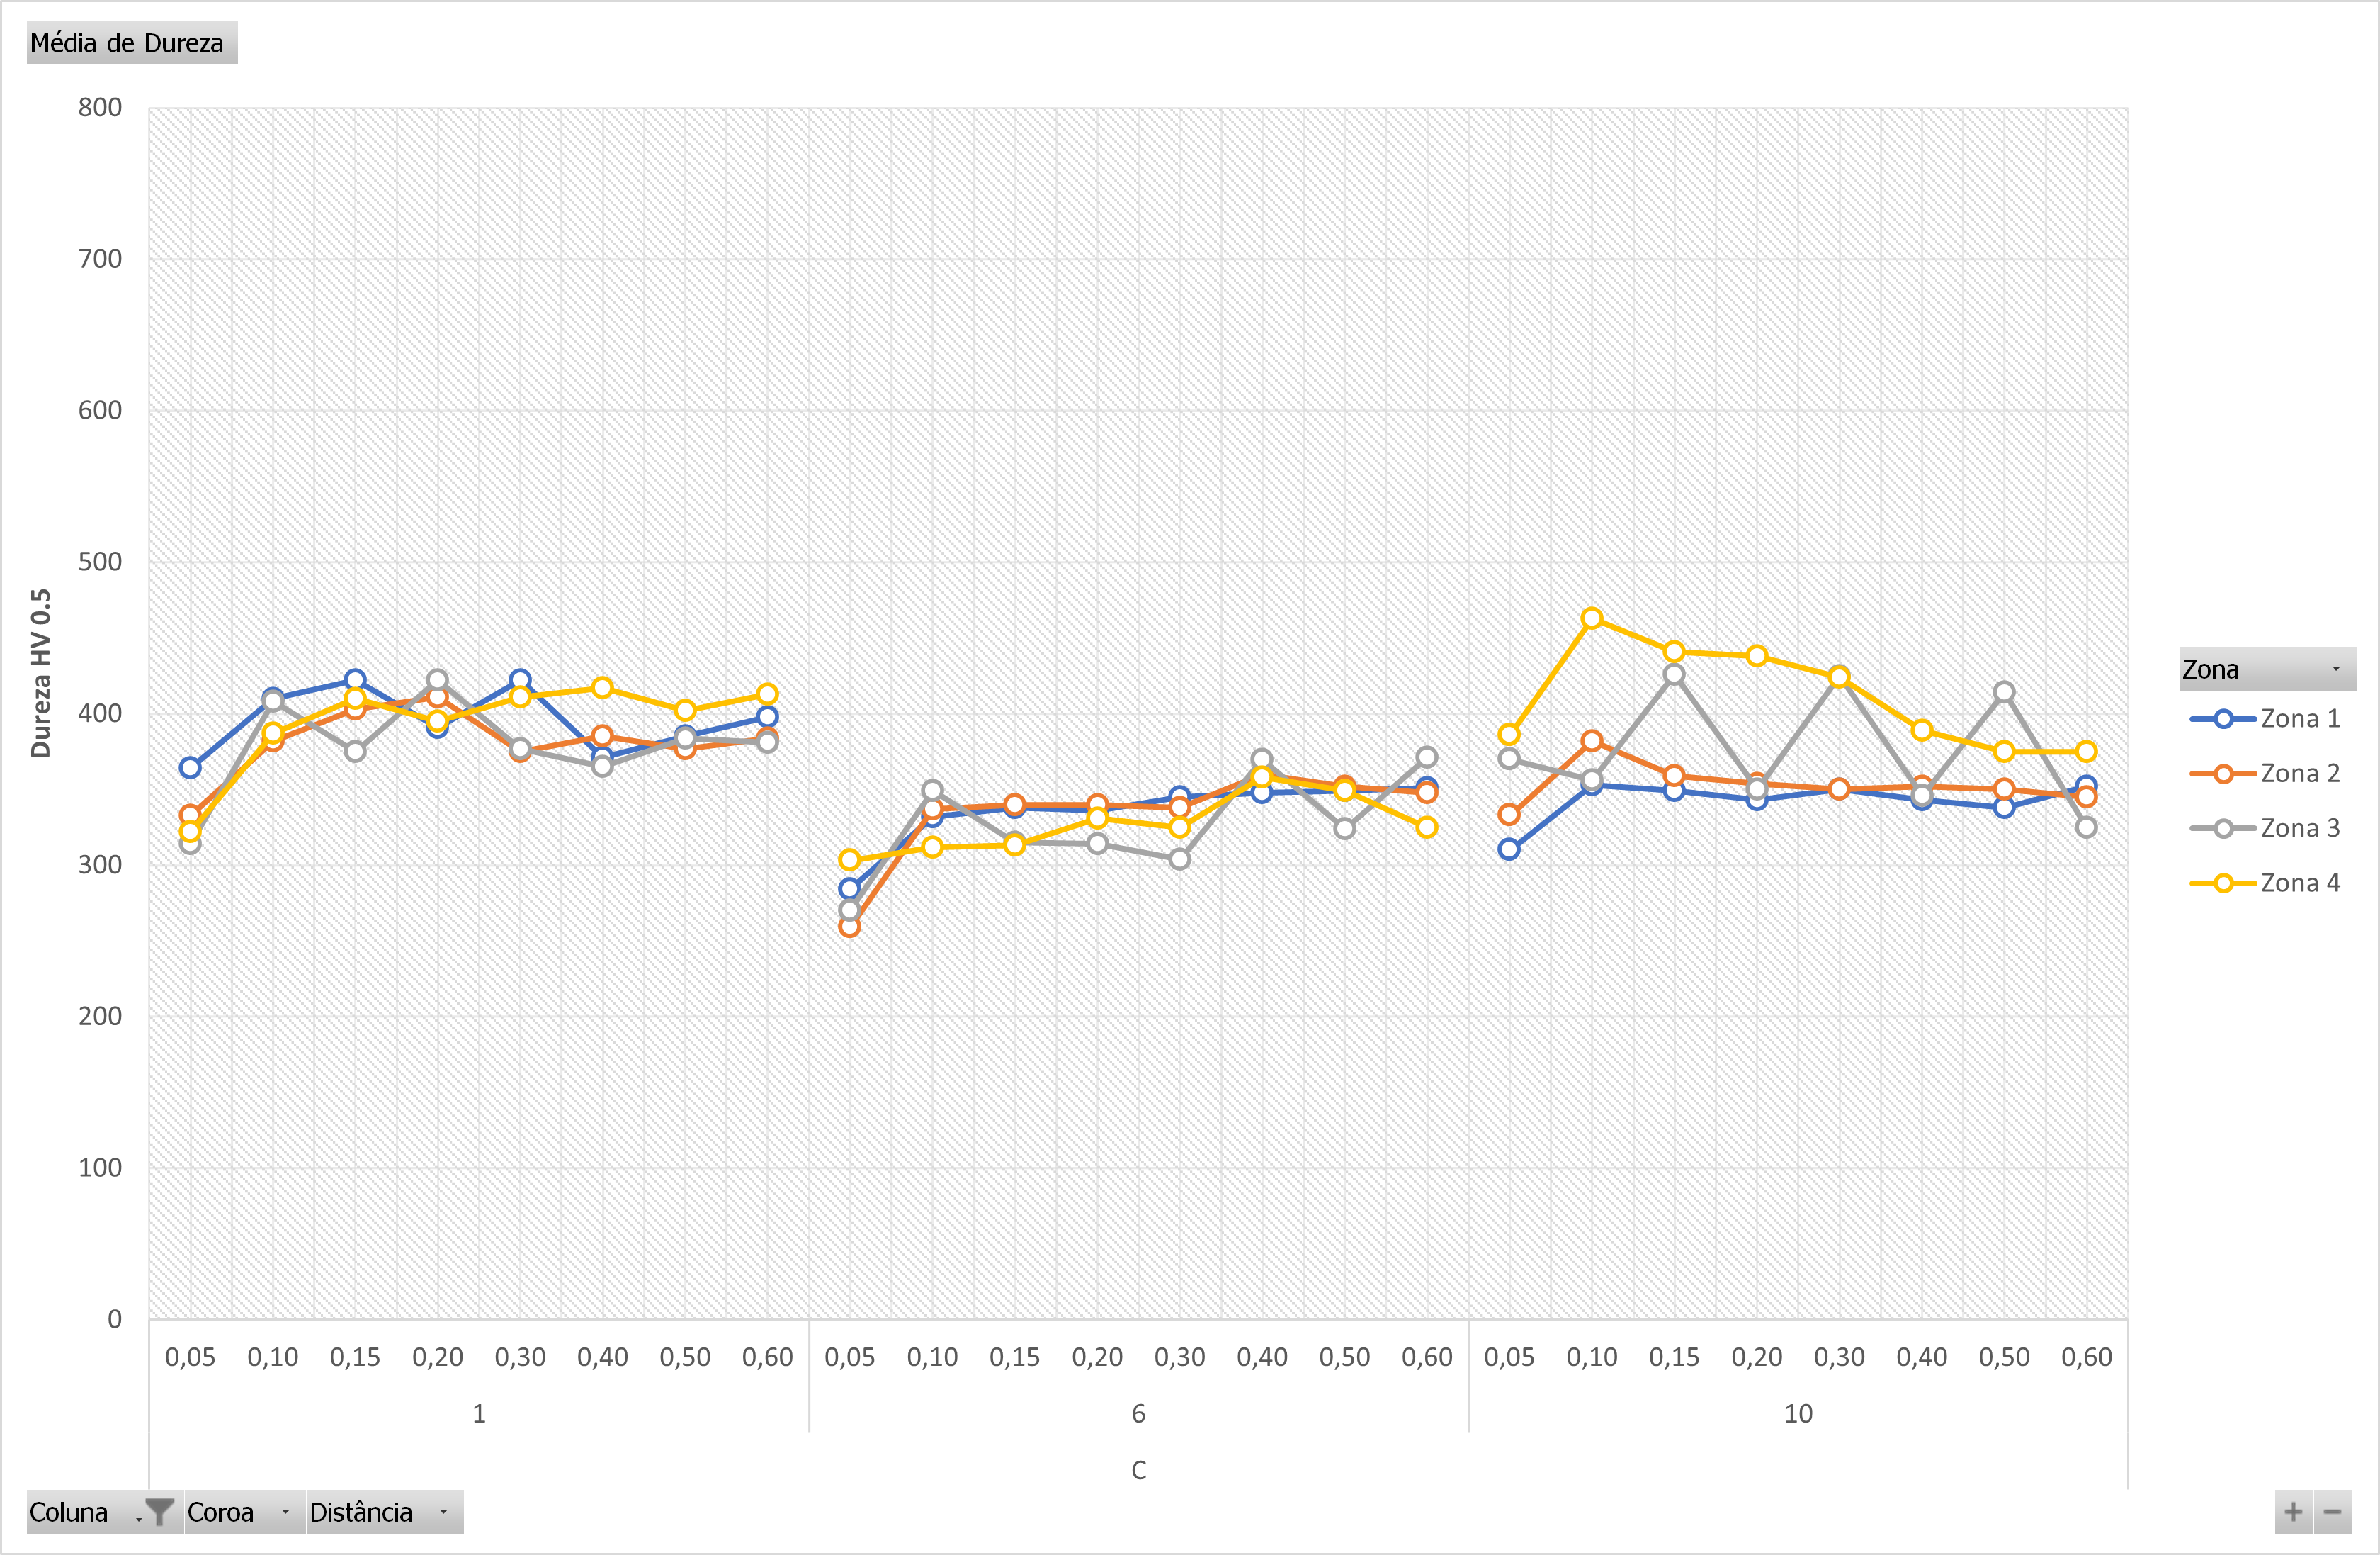
\includegraphics[width = 0.9\textwidth]{Figures/Cap4/Grafico_4_Zonas_P.png}
        \caption{}
        \label{fig:resultados_Tampa_P}
    \end{subfigure}%
    \begin{subfigure}{.4\textwidth}
        \centering
        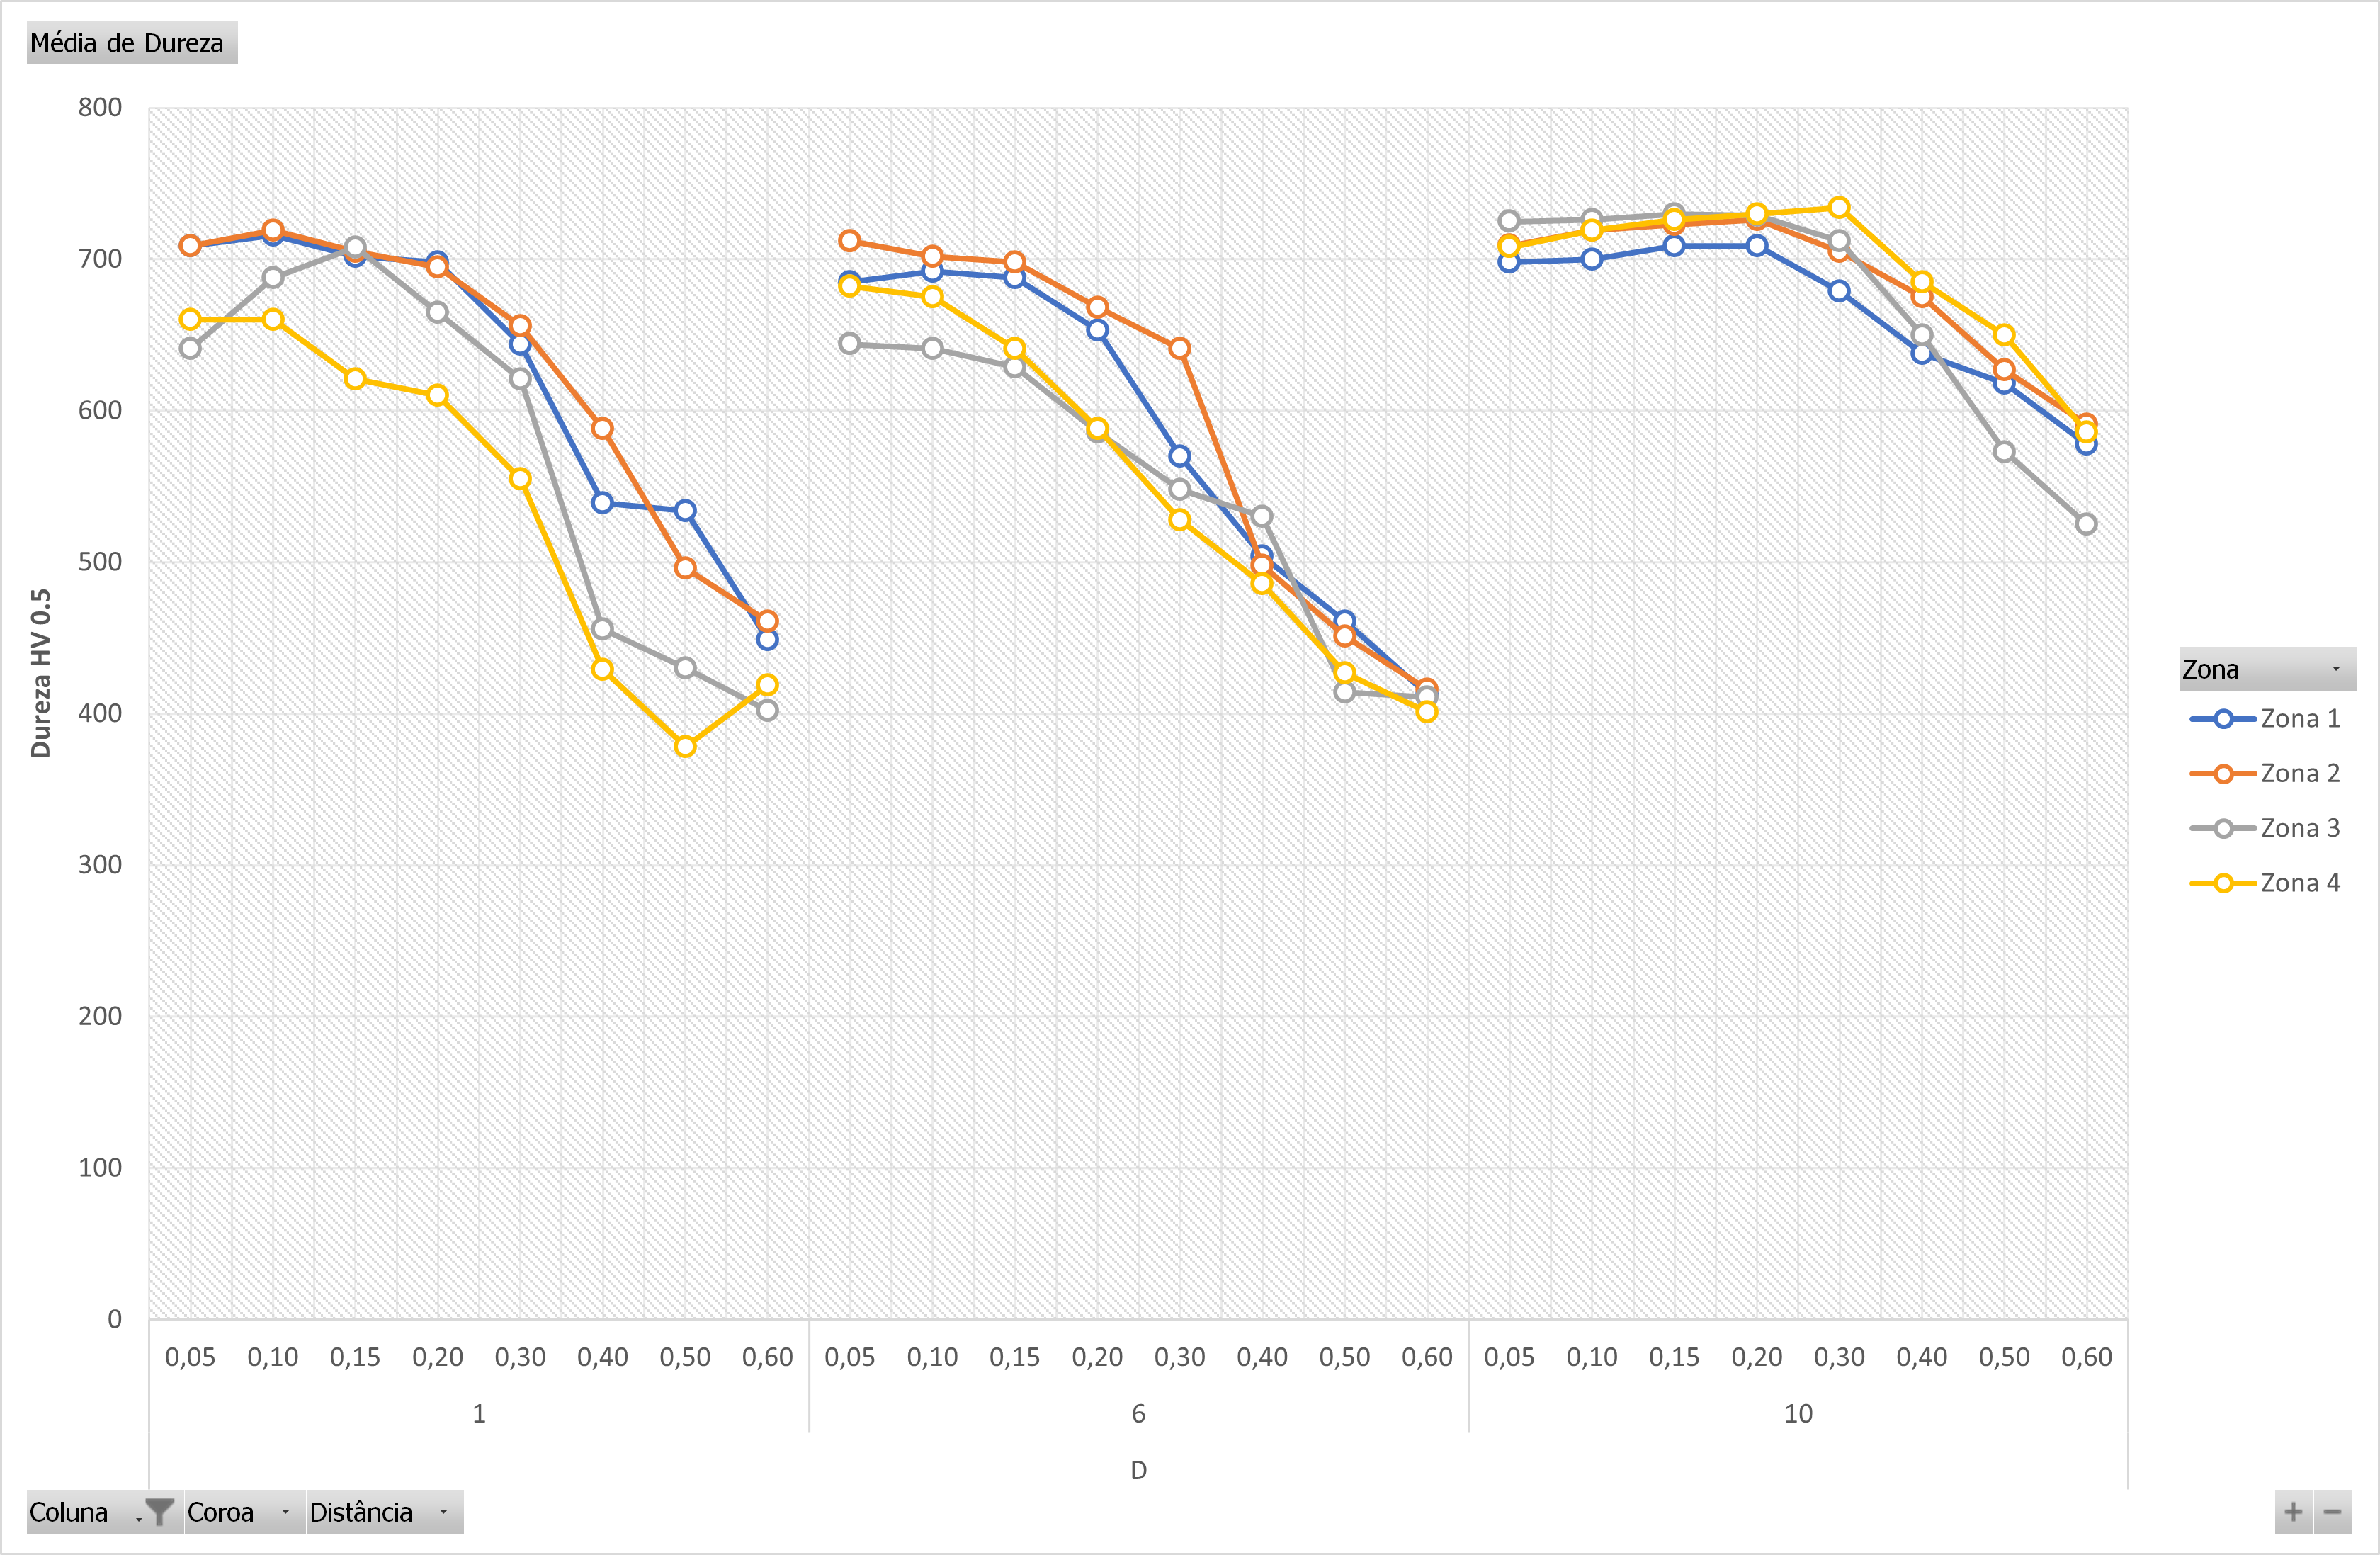
\includegraphics[width = 0.9\textwidth]{Figures/Cap4/Grafico_4_Zonas_ST.png}
        \caption{}
        \label{fig:resultados_ST}
    \end{subfigure}
    \caption[Filiações de dureza das quatro zonas na roda de coroa DB45 Nº 1]%
    {Gráficos das filiações de dureza das quatro zonas nas rodas de coroa protegidas por tampa Y, protegidas por tampa O, e protegida por tampa P, e sem tampa de proteção, respetivamente.}
\end{figure}
%%%%%%%%%%%%%%%%%%%%%%%%%%%%%%%%%%%%%%%%%%%%%%%%%%%%%%%%%%%%%%%%%%%%%%%%%%%%%
\newpage
\par
Observa-se claramente uma redução nos níveis de dureza em todos os tipos de ferramentas de proteção com tampa. No entanto, na ferramenta sem tampa, que protege apenas a parte inferior, não se observa uma alteração significativa nos níveis de dureza. Isso confirma duas teorias. Primeiro, que o uso de uma tampa é essencial para o funcionamento do sistema. E segundo, que a geometria da tampa não tem impacto significativo no resultado da proteção. É importante mencionar que não foi proposta uma solução que dispensasse a proteção na parte inferior, uma vez que o fluido de têmpera é carregado de baixo para cima no tanque de têmpera, o que poderia resultar na remoção da tampa pelo fluido de têmpera e possíveis danos ao sistema de têmpera. Novamente, nas Figuras \ref{fig:resultados_4T_dent}, não são observadas alterações significativas nas durezas do dentado em nenhuma das soluções propostas.
%%%%%%%%%%%%%%%%%%%%%%%%%%%%%%%%%%%%%%%%%%%%%%%%%%%%%%%%%%%%%%%%%%%%%%%%%%%%%
\begin{figure}[htb]
    \centering
    \begin{subfigure}{.4\textwidth}\
        \centering
        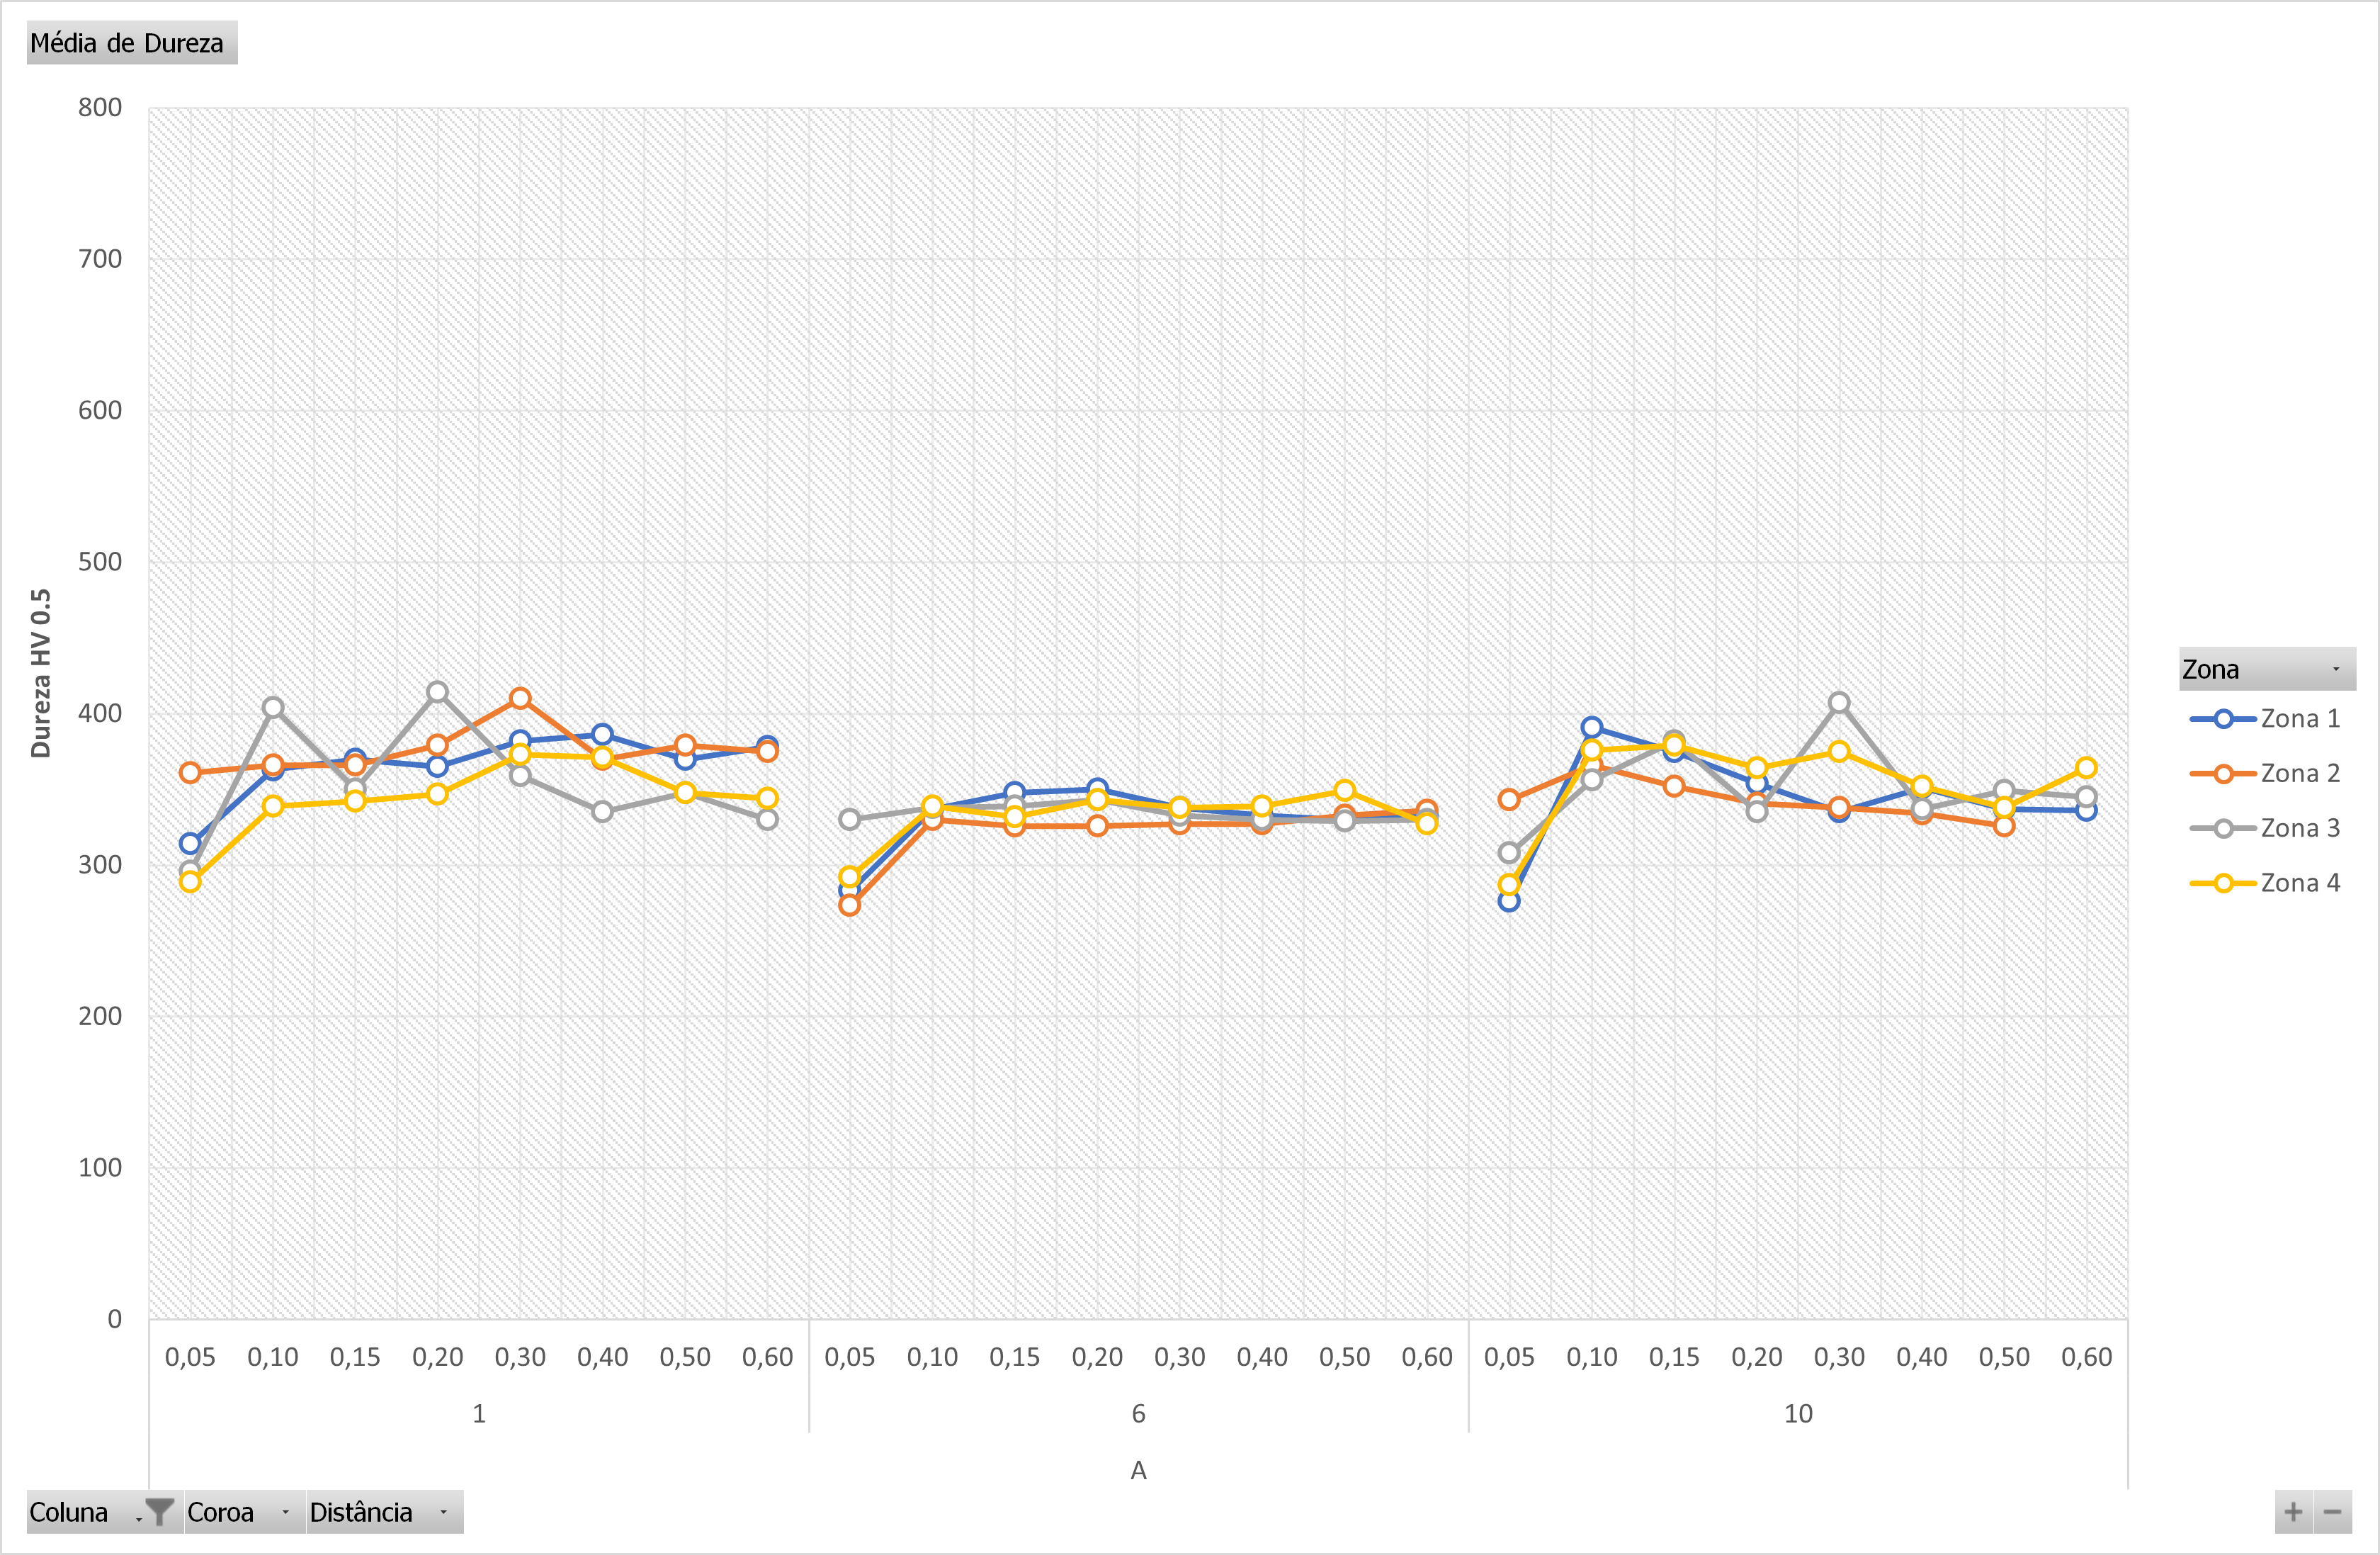
\includegraphics[width = 0.9\textwidth]{Figures/Cap4/Grafico_4_Zonas_Y.png}
        \caption{}
        \label{fig:resultados_Tampa_Y_dent}
    \end{subfigure}%
    \begin{subfigure}{.4\textwidth}
        \centering
        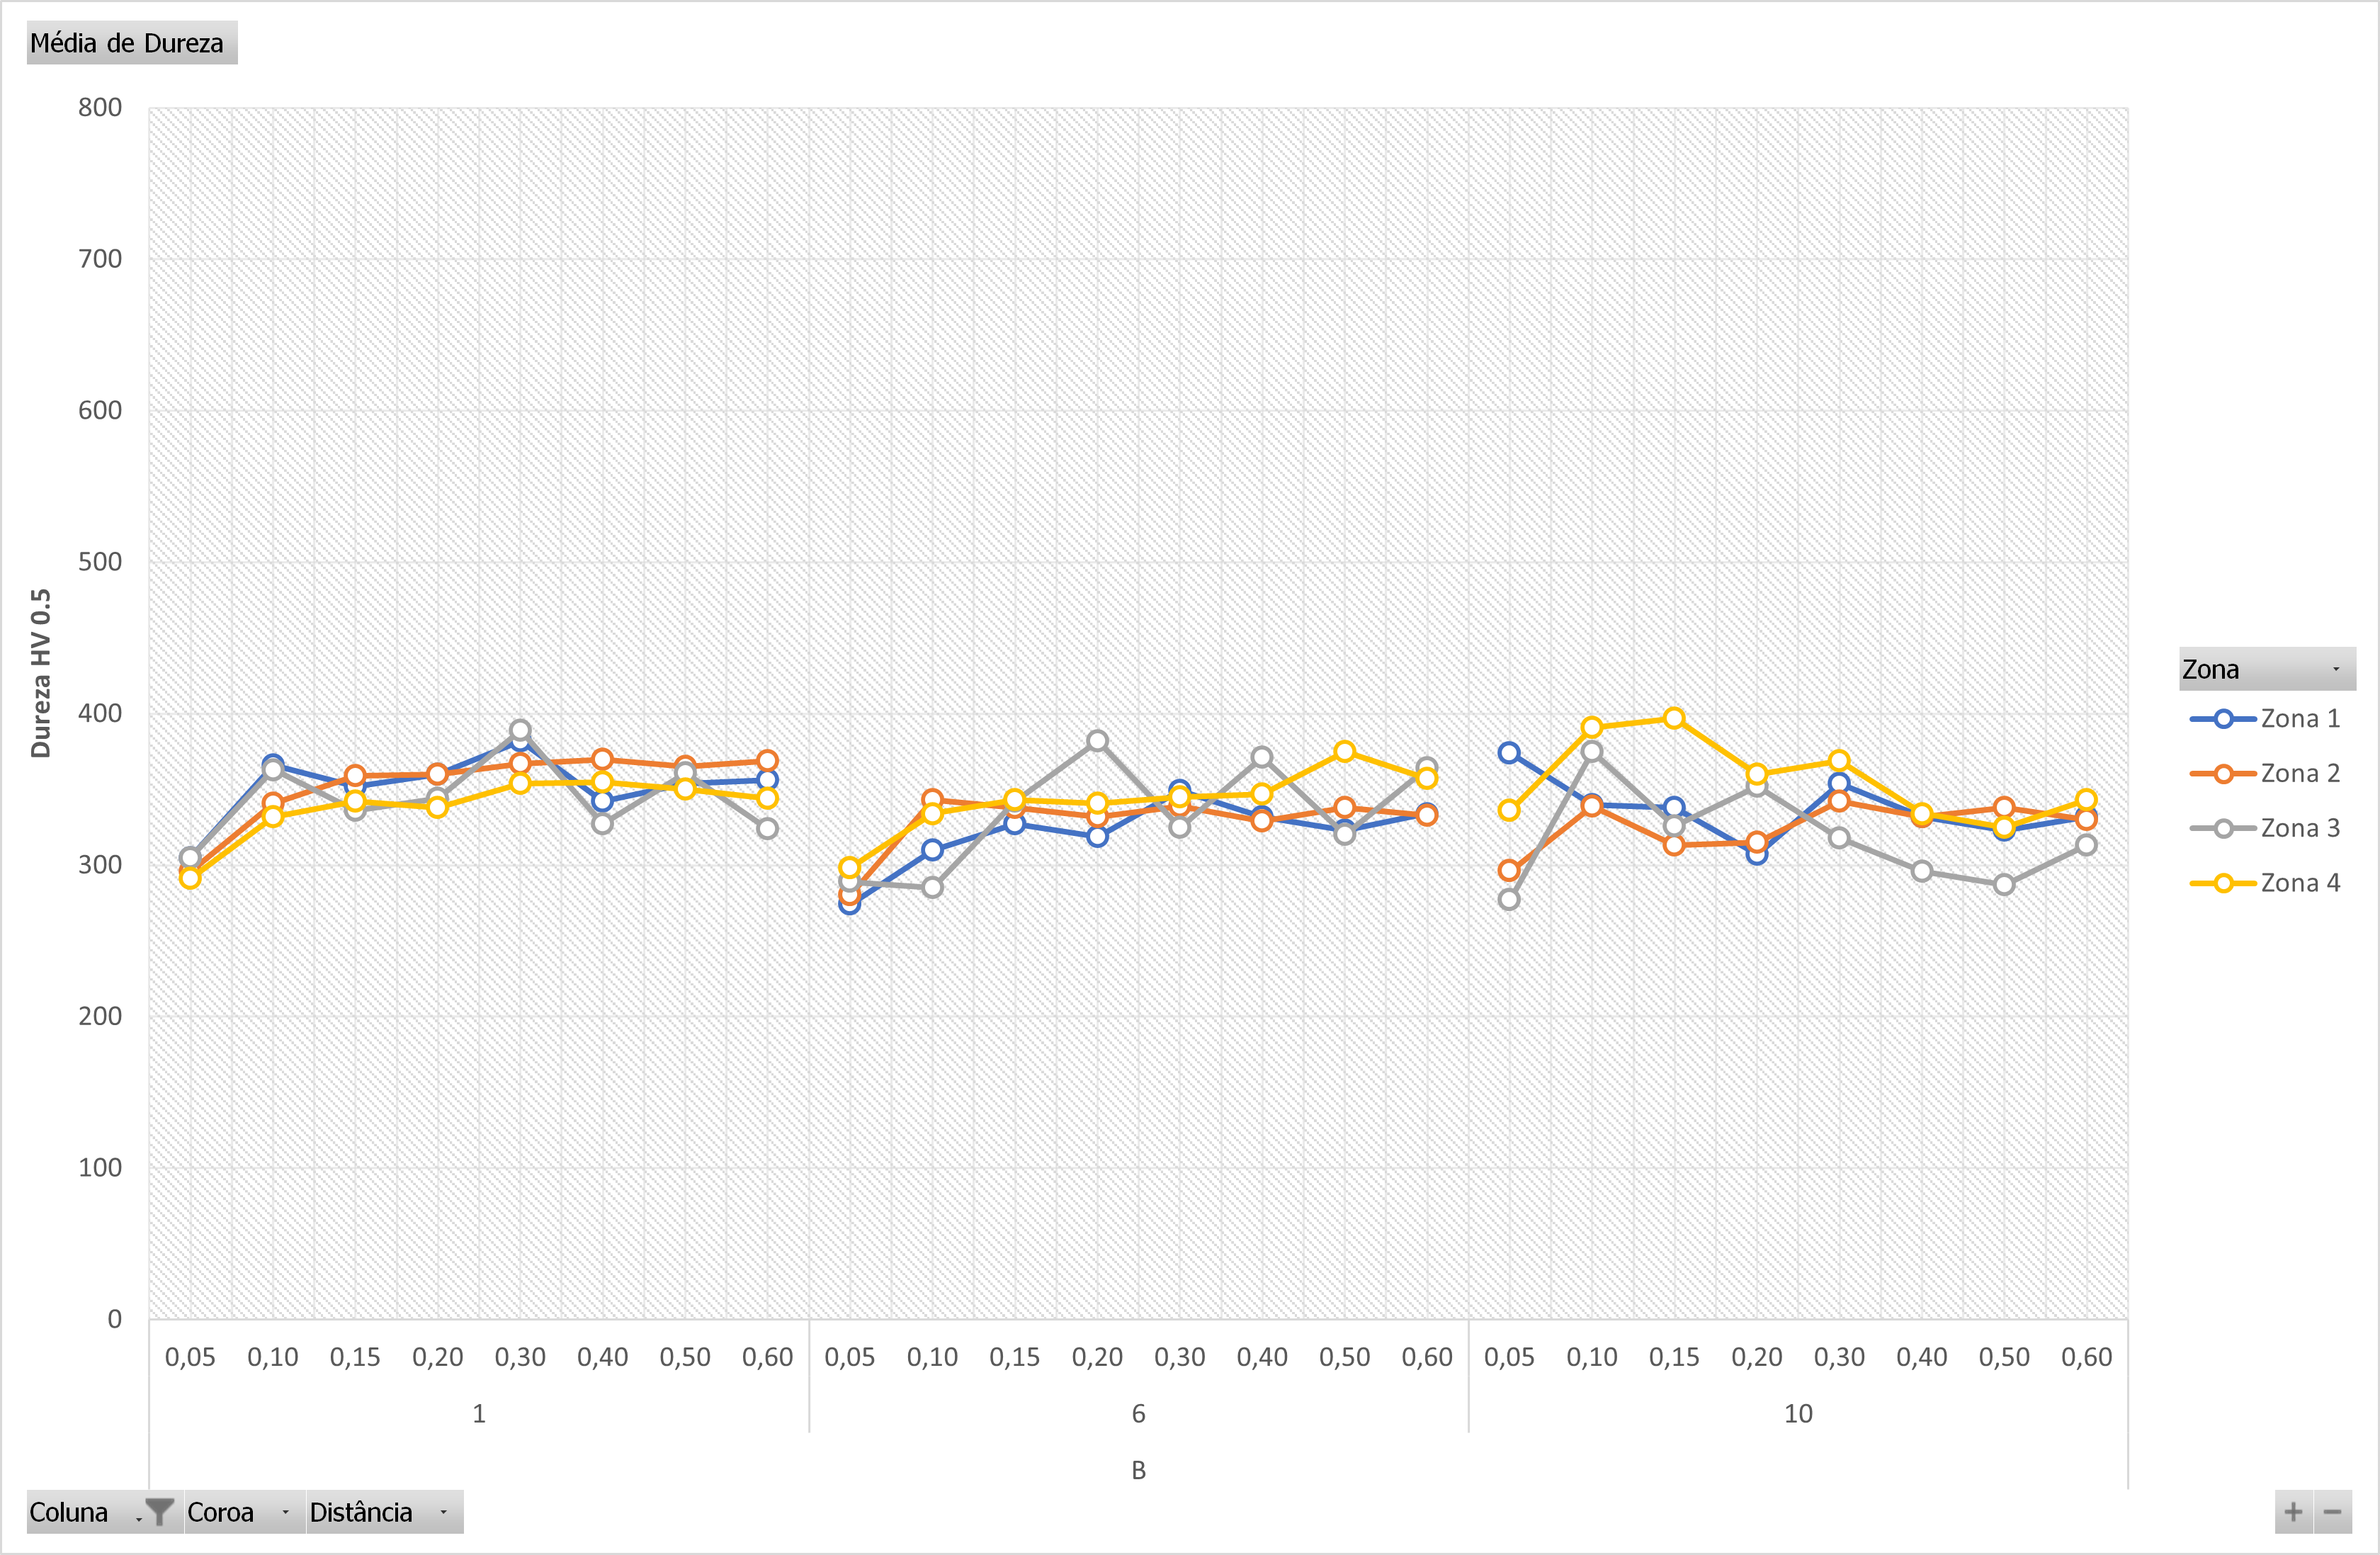
\includegraphics[width = 0.9\textwidth]{Figures/Cap4/Grafico_4_Zonas_O.png}
        \caption{}
        \label{fig:resultados_Tampa_O_dent}
    \end{subfigure}
    \begin{subfigure}{.4\textwidth}\
        \centering
        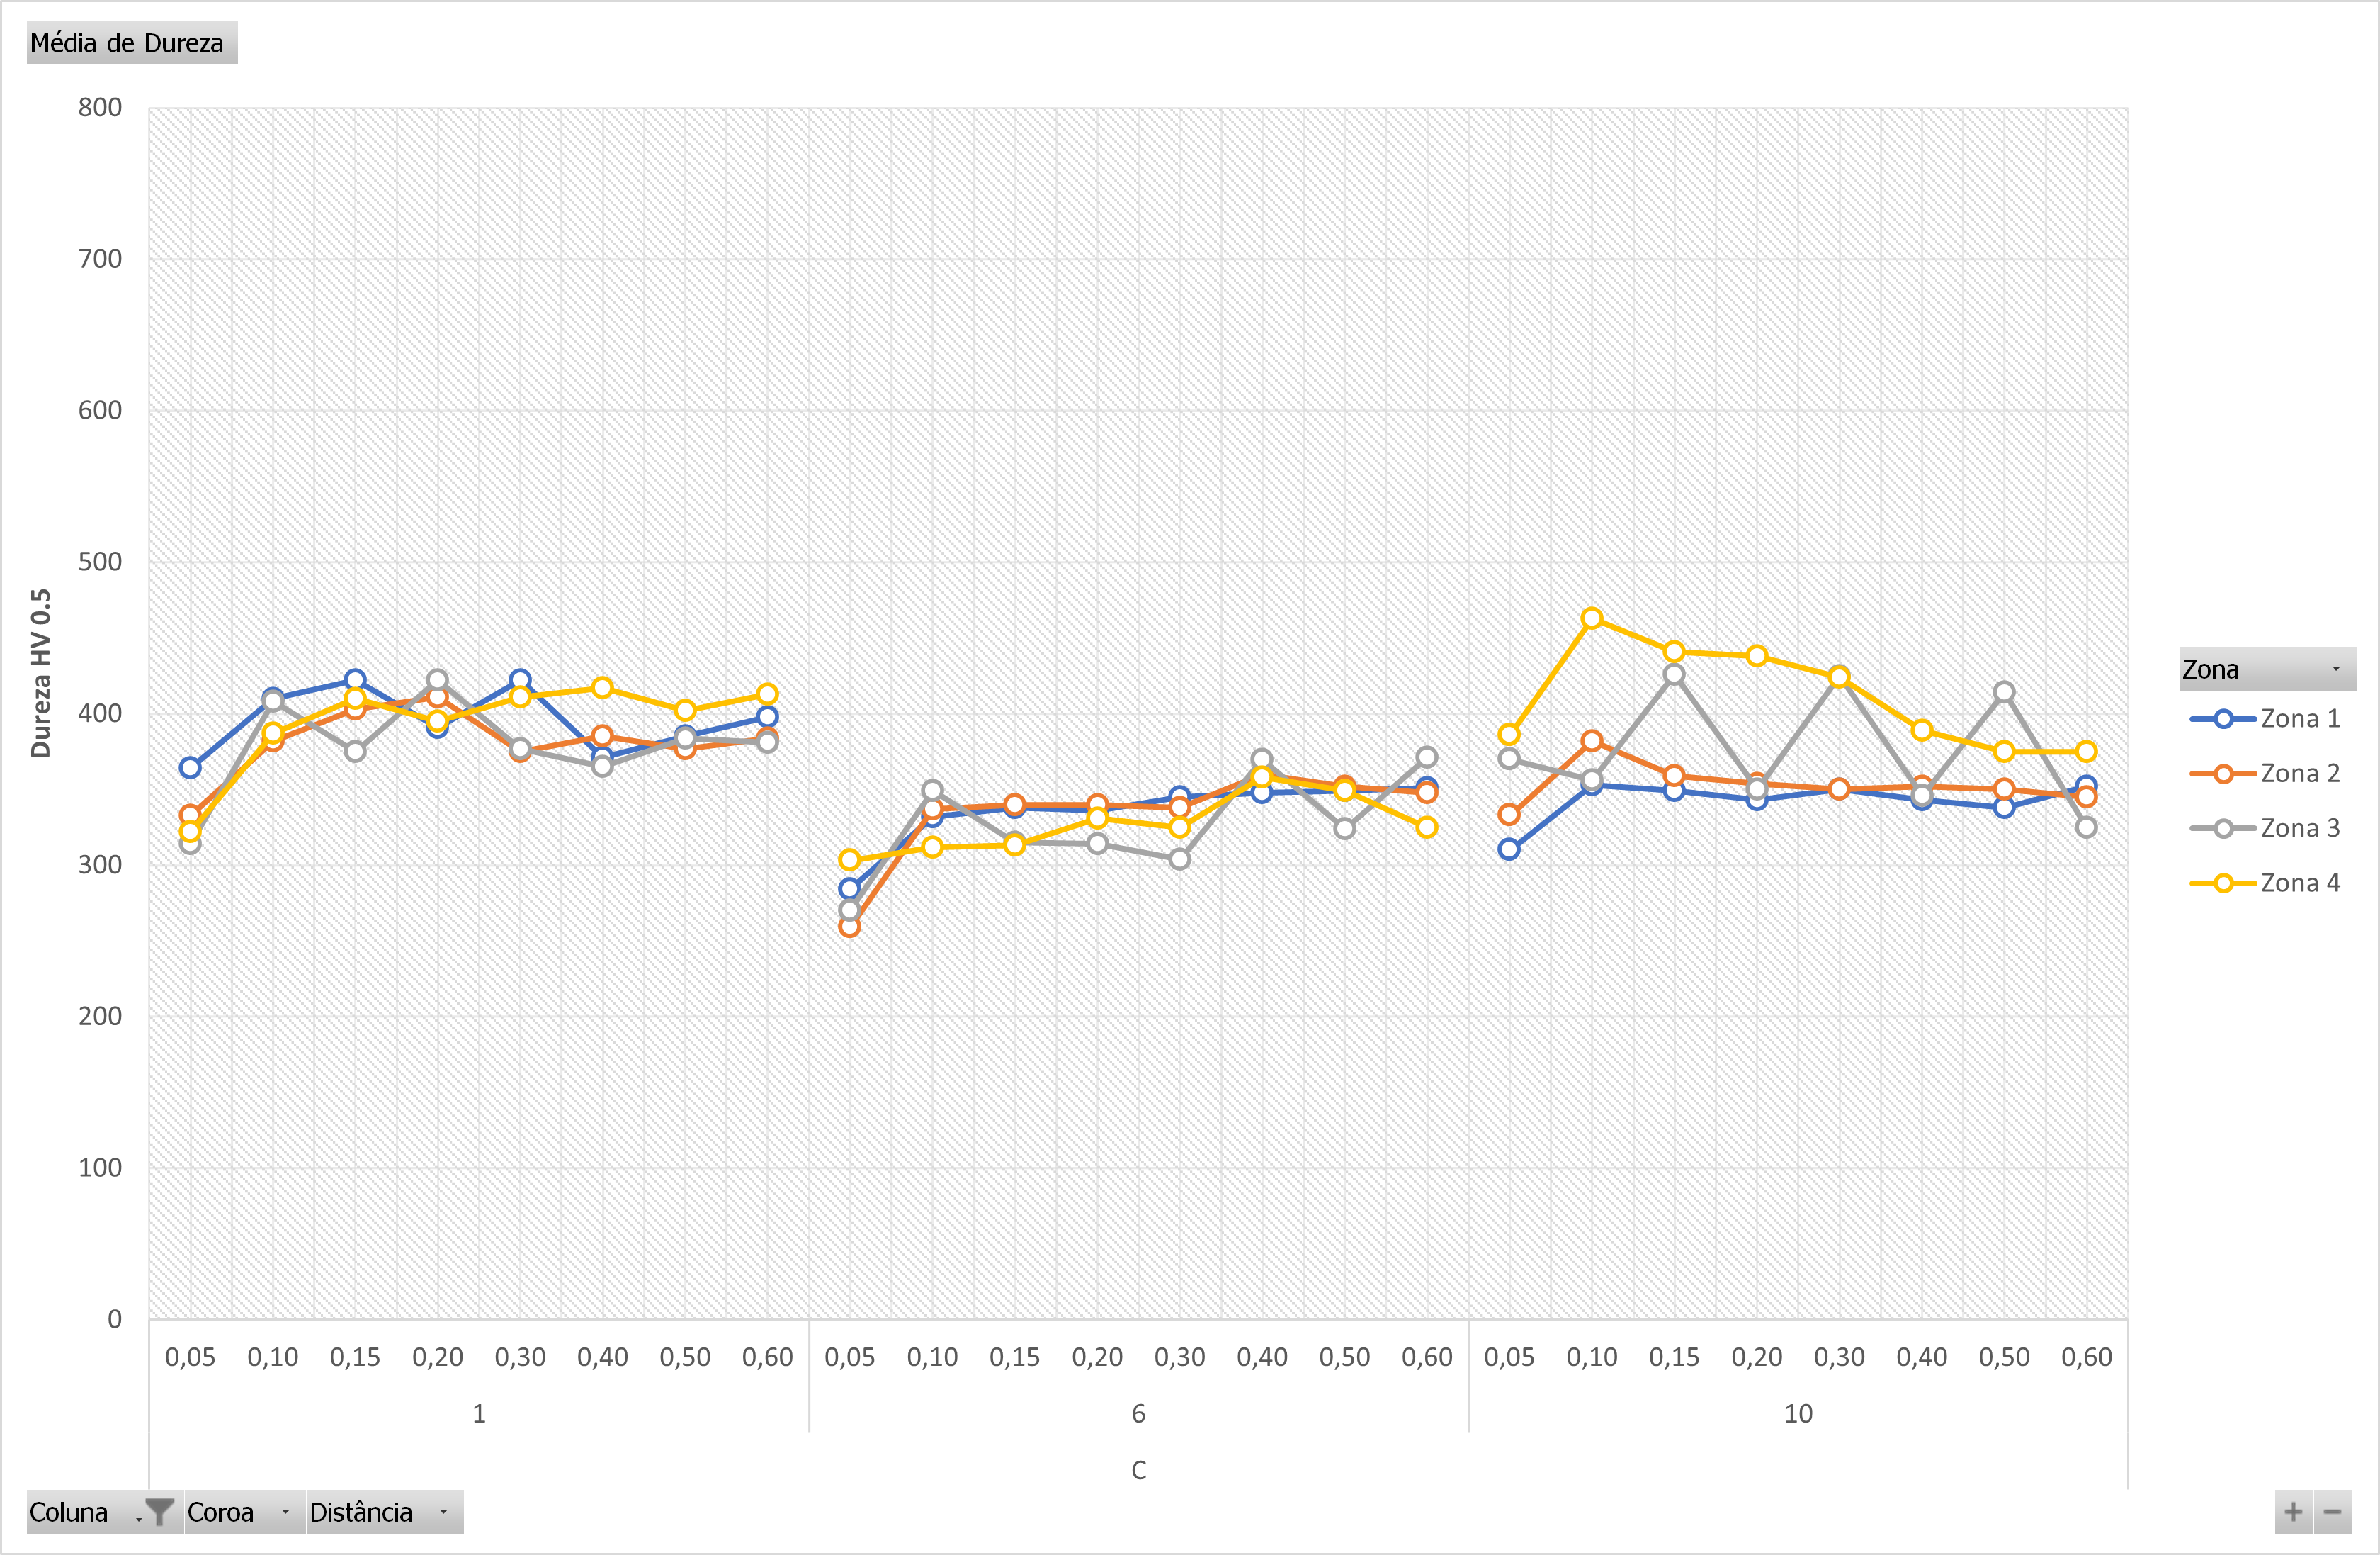
\includegraphics[width = 0.9\textwidth]{Figures/Cap4/Grafico_4_Zonas_P.png}
        \caption{}
        \label{fig:resultados_Tampa_P_dent}
    \end{subfigure}%
    \begin{subfigure}{.4\textwidth}
        \centering
        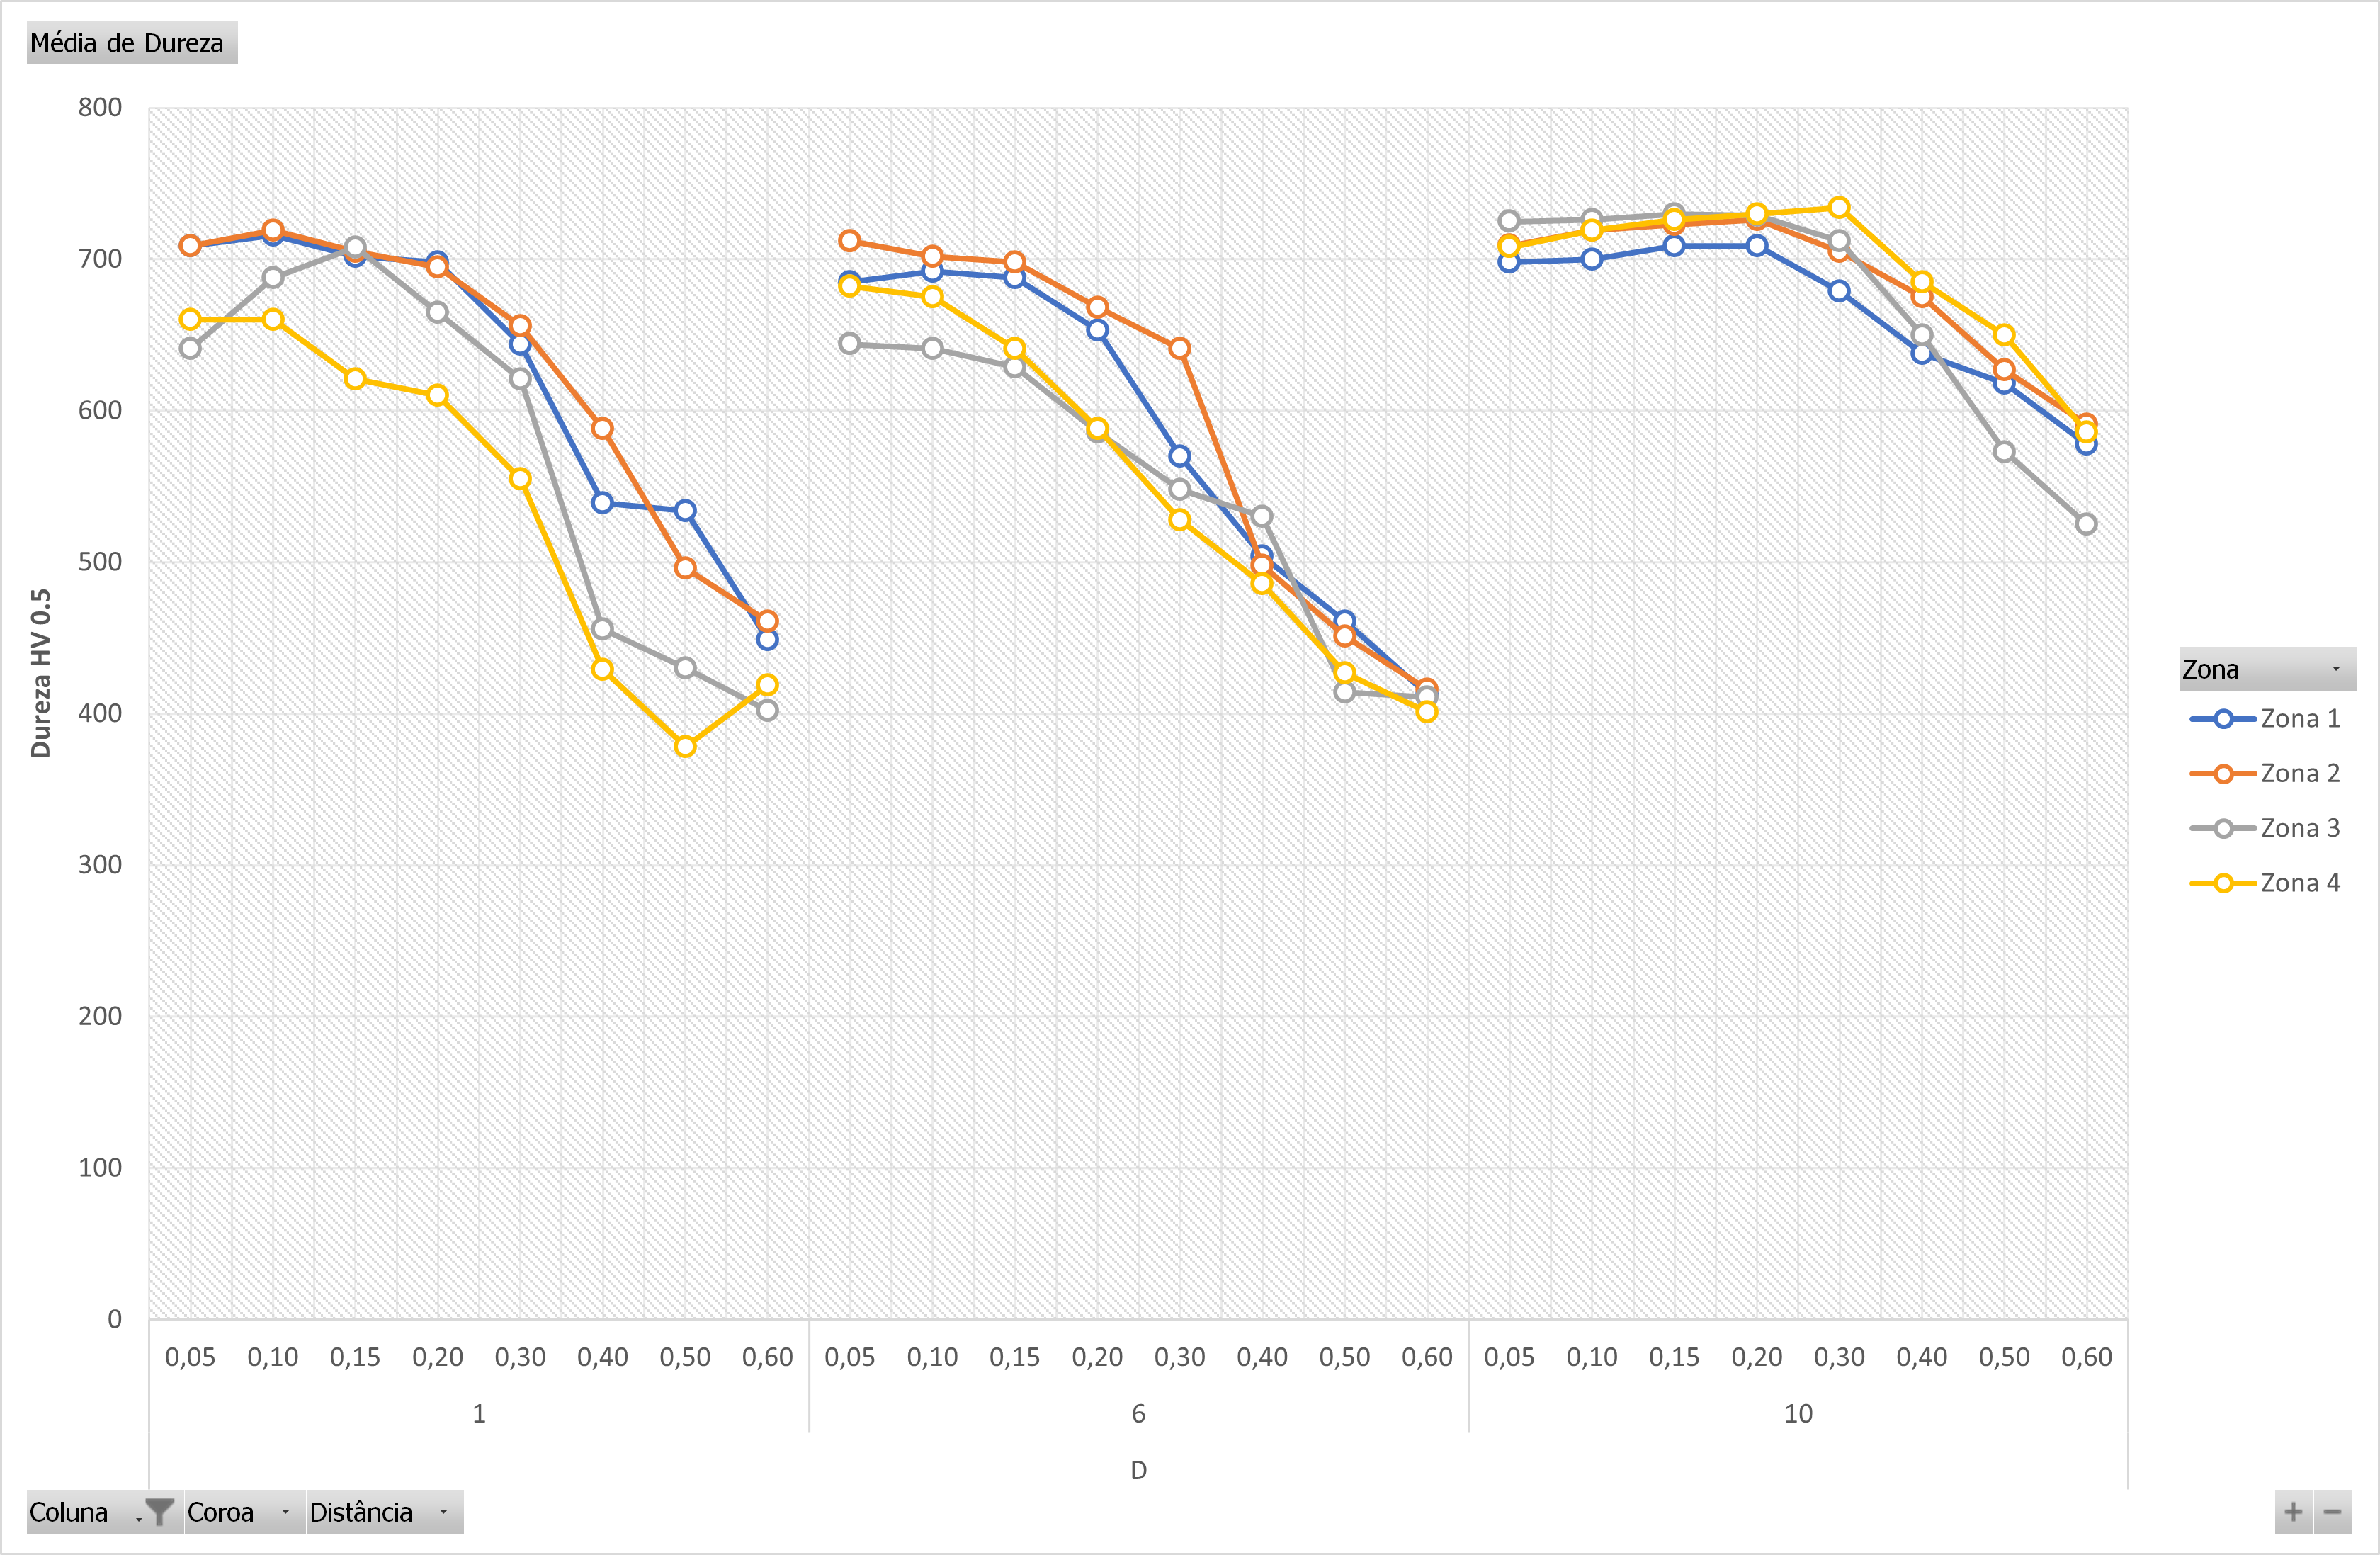
\includegraphics[width = 0.9\textwidth]{Figures/Cap4/Grafico_4_Zonas_ST.png}
        \caption{}
        \label{fig:resultados_ST_dent}
    \end{subfigure}
    \caption[Filiações de dureza das quatro zonas na roda de coroa DB45 Nº 1]%
    {Gráficos das filiações de dureza das quatro zonas nas rodas de coroa protegidas por tampa Y, protegidas por tampa O, e protegida por tampa P, e sem tampa de proteção, respetivamente.}
    \label{fig:resultados_4T_dent}
\end{figure}
%%%%%%%%%%%%%%%%%%%%%%%%%%%%%%%%%%%%%%%%%%%%%%%%%%%%%%%%%%%%%%%%%%%%%%%%%%%%%
\section{Resultados da Espectroscopia} \label{sec:resultados_espectroscopia}
